% compile-latex options: --jobname archi
% compile-latex options: --jobname poly
% compile-latex options: --jobname exo
% compile-latex options: --jobname prof

\documentclass{iutv2013}
\usepackage{listings}
\usepackage{caption}
\DeclareCaptionFont{white}{\color{solarizedRebase3}}
\DeclareCaptionFormat{listing}{\colorbox{solarizedRebase00}{\parbox{\textwidth}{\hspace{15pt}#3}}}
\captionsetup[lstlisting]{format=listing,labelfont=white,textfont=white, singlelinecheck=false, margin=0pt, font={bf,footnotesize}}
\usepackage{realboxes}

\lstdefinelanguage{JavaScript}{
  sensitive=true,
  keywords={break, else, case, finally, return, catch, for, switch, while, continue, default, if, throw, in, try, do},
  keywords=[2]{this, true, false, null, instanceof, typeof, new, void, with, function, delete, var},
  keywords=[3]{console,window,arguments,document,node,$,jQuery},
  % $ Error was removed due to case insensitivity bug
  sensitive=false,
  comment=[l]{//},
  morecomment=[s]{/*}{*/},
  morestring=[b]',
  morestring=[b]"
}
\lstset{literate=%
  {Ö}{{\"O}}1
  {à}{{\`a}}1
  {é}{{\'e}}1
  {Ä}{{\"A}}1
  {Ü}{{\"U}}1
  {ß}{{\ss}}2
  {ü}{{\"u}}1
  {ä}{{\"a}}1
  {ö}{{\"o}}1
  {ö}{{\"o}}1
  {ê}{{\^e}}1
  {â}{{\^a}}1
}
\lstset{
  language=Javascript,
  numbers=left,
  basicstyle=\fontfamily{qhvc}\footnotesize,
  numberstyle=\fontfamily{qhvc}\tiny,
  keywordstyle=\color{red}\bfseries,
  keywordstyle=[2]\color{solarizedRed}\bfseries,
  keywordstyle=[3]\color{solarizedRebase3}\bfseries,
  identifierstyle=\color{solarizedRebase3},
  stringstyle=\fontfamily{qhvc}\color{solarizedBlue},
  commentstyle=\fontfamily{qhvc}\color{solarizedMagenta},
  numbersep=5pt,
  tabsize=2,
  extendedchars=true,
  breaklines=true,
  frame=b,
  columns=fullflexible,
  showspaces=false,
  showtabs=false,
  xleftmargin=10pt,
  framexleftmargin=10pt,
  framexrightmargin=5pt,
  framexbottommargin=1pt,
  showstringspaces=false,
  % escapeinside={}{}
}

% Background
\usepackage{etoolbox,ifthen}

\tikzstyle{highlighter} = [solarizedRebase3,fill=solarizedYellow,dashed,opacity=.2]
\tikzstyle{highlightergreen} =[highlighter,fill=solarizedGreen,solid,line width=0.5pt,rounded corners=3pt]
\tikzstyle{highlighterblue} =[highlighter,fill=solarizedBlue,solid,line width=0.5pt]
\tikzstyle{highlightermagenta} =[highlighter,fill=solarizedMagenta,solid,line width=0.5pt]
\pgfdeclarelayer{foreground}
\pgfdeclarelayer{background} 
\pgfsetlayers{background,main,foreground} 
\xdef\highlighter{highlighter}

\newcounter{highlight}[page]
\newcommand{\bh}[0]{%
  \stepcounter{highlight}%
  \tikz[remember picture, overlay]{%
    \coordinate (begin highlight \arabic{highlight}) at (-.1em,-.2\baselineskip);%
  }}
\newcommand{\eh}[0]{%
  \tikz[remember picture, overlay]{%
    \coordinate (end highlight \arabic{highlight}) at (.1em,.8\baselineskip);;%
    \draw[\highlighter] (begin highlight \arabic{highlight}) rectangle (end highlight \arabic{highlight});
  }}

\makeatletter %   Redefine macros from listings package:
\renewcommand\lstinline[1][]{%
    \leavevmode\bgroup\bh\aftergroup\eh % \hbox\bgroup --> \bgroup
      \def\lst@boxpos{b}%
      \lsthk@PreSet\lstset{flexiblecolumns,#1}%
      \lsthk@TextStyle
      \@ifnextchar\bgroup{\afterassignment\lst@InlineG \let\@let@token}%
                         \lstinline@}
\makeatother

\def\event#1{\bgroup\edef\highlighter{highlightergreen}\fontfamily{qhvc}\normalsize\bh#1\eh[highlightergreen]\egroup}
\long\def\shortjs{\edef\highlighter{highlightergreen}\lstinline[basicstyle=\fontfamily{qhvc}\normalsize]}
\def\shorthtml{\edef\highlighter{highlightermagenta}\lstinline[basicstyle=\fontfamily{qhvc}\normalsize,language=HTML]}
\def\shortphp{\edef\highlighter{highlighterblue}\lstinline[basicstyle=\fontfamily{qhvc}\normalsize,language=PHP]}
% \catcode`\$=11 %$

\usetikzlibrary{fadings,decorations.text}

\subtitle{Cours complet}
\usepackage{arabtex}

\begin{document}
\beamertitle
\begin{frame}{Organisation du module}
  \begin{alertblock}{Remerciements}
    \begin{itemize}
    \item Les cours et exercices de ce module sont directement inspirés
      des documents de \textbf{M. Bosc}, \textbf{J.-C. Dubacq} et \textbf{G. Santini}.
    \item D'autres intervenants ont participé à l'élaboration des supports.
    \end{itemize}
  \end{alertblock}
  \begin{block}{Les enseignements}
    \begin{itemize}
    \item 12 sessions de 4h et du travail personnel \dots
    \item 6 sessions pour la présentation générale du système
      d'exploitation Linux,
    \item 6 sessions pour la théorie de base du codage informatique 
    \end{itemize}
  \end{block}
  \begin{alertblock}{Votre présence est obligatoire}
    \begin{itemize}
    \item Contrôle des présences.
    \item Rapport des absences.
    \end{itemize}
  \end{alertblock}
  \begin{block}{L'évaluation}
    \begin{itemize}
    \item Une composition après la sixième session (sur papier ou sur
      ordinateur).
    \item Une composition à la fin du module (sur papier ou sur
      ordinateur).
    \end{itemize}
  \end{block}
\end{frame}

\endinput

\section{La machine}
\subsection{L'histoire des ordinateurs}
\subsection{Le processeur}
\subsection{La mémoire}

% Local Variables:
% TeX-master: "archi00"
% TeX-PDF-mode: t
% fill-column: 78
% coding: utf-8-unix
% mode-require-final-newline: t
% mode: latex
% mode: flyspell
% ispell-local-dictionary: "francais"
% End:

\section{Représenter une information}
\subsection{Du sens à la mesure}
\begin{exercice}
  \begin{exercicelet}{Qu'est-ce que l'information}
    \begin{enumerate}
    \item Proposez différents symbolismes utilisés pour noter un
      nombre. Donnez l'exemple de leur notation avec le nombre 9. Donnez des
      inconvénients de votre méthode.
    \item Travaillez en paire (ou triplettes). Proposez une méthode pour
      transmettre d'une personne à une autre le résultat d'un lancer de dé
      (lancer caché par la première personne, la deuxième doit pouvoir énoncer
      le résultat). Votre méthode fonctionne-t-elle si le dé comporte 20
      faces ? Et si le dé est à six faces mais étiqueté par des couleurs ?
    \end{enumerate}
  \end{exercicelet}
\end{exercice}
\begin{frame}{Qu'est-ce qu'une information ?}
  \begin{block}{Information}
    Une information est une donnée que l'on peut interpréter pour se
    construire une représentation du monde sur laquelle on peut agir.
  \end{block}
  \begin{itemize}
  \item[\dialoginformation] Claude Shannon a été l'un des premiers à
    définir l'information comme une quantité mesurable.
  \item[\dialogwarning] L'information de Shannon n'est pas associé au
    sens ou à la cognition.
  \item Il s'est intéressé à quantifier des sources aléatoires
  \item L'information diminue l'incertitude sur une source aléatoire
  \item On mesure donc la quantité d'information relative à un événement
  \item Par exemple, si on a six possibilités pour un dé, l'information
    permet de savoir quelle face; ou au moins d'éliminer des
    possibilités
  \end{itemize}
\end{frame}
\begin{frame}{La vision cognitive de l'information}
  \begin{itemize}
  \item[\dialogerror] On ne sait pas mesurer le \emph{sens} des choses.
  \item[\dialoginformation] Une même information peut avoir plusieurs représentations très distinctes.
  \item[\dialogsystem] Le nombre quatorze: 14 ou XIV ou IIIIIIIIIIIIII
  \item[\dialoginformation] Une même donnée peut être interprétée de plusieurs façons → informations très distinctes.
  \item[\dialogsystem] Inversement: XIV est un mot ou un nombre
  \end{itemize}
  \centerline{
    \begin{tikzpicture}
      \tikzstyle{every node}=[fill=solarizedRebase02,draw=solarizedRebase0,rounded corners]
      \tikzstyle{data}=[color=solarizedRed,every node]
      \tikzstyle{xlabel}=[color=solarizedMagenta,fill opacity=30,text opacity=1,every node]
      \tikzstyle{snaky}=[decorate,normally,decoration={snake,pre length=5mm}]
      \tikzstyle{normally}=[very thick]
      \tikzstyle{cloudy}=[color=solarizedGreen,every node]
      \node [cloudy] (a) at (0,2) {Concept};
      \node [cloudy] (b) at (6,2) {Concept}
      edge [<-,snaky] node[xlabel,below] {fonction} (a);
      \node [data] (c) at (0,0) {Donnée}
      edge  [<-,normally] node[xlabel] {représentation} (a) (a);
      \node [data] (d) at (6,0) {Donnée}
      edge  [<-,normally] node[xlabel,above] {algorithme}(c)
      edge  [->,normally] node[xlabel] {interprétation} (b);
    \end{tikzpicture}
  }
\end{frame}
\begin{frame}{L'information digitale}
  \begin{itemize}
  \item Les systèmes d'informations (et les ordinateurs en particulier)
    ne sont pas équipés pour traiter n'importe quel type de données.
  \item Toutes les informations sont représentées sous forme de nombres
    pour être traitées par les ordinateurs.
  \item Le monde réel est \emph{analogique}, la représentation des
    ordinateurs est \emph{numérique} (ou \emph{digitale}).
  \item Nous considérerons que nous avons toujours affaire à des
    problèmes représentables par des nombres.
  \end{itemize}
\end{frame}

\begin{exercice}
  \begin{exercicelet}{Digital ou analogique?}
    Est-ce que les données suivantes sont digitales ou analogiques :
    \begin{itemize}
    \item Le fait d'avoir un rendez-vous à une certaine heure un certain jour
    \item La pression de l'air
    \item Le résultat (stable) d'un dé
    \item Votre nom de famille
    \item Votre nombre de frères et sœurs
    \item Votre taille
    \item La couleur de vos yeux
    \end{itemize}
  \end{exercicelet}
\end{exercice}
\subsection{Mesurer l'information}
\begin{frame}[label=mesure]{L'information mesurée}
  \begin{block}{bit}
    Le bit est la quantité d'information qui permet de choisir
    complètement entre deux issues distinctes d'un événement.

    Le mot de \emph{bit} est l'abréviation de \emph{binary digit}.
  \end{block}
  \begin{block}{Mesure de l'information}
    Pour exprimer $k$ choix possibles distincts, il faut
    $\left\lceil\log_2(k)\right\rceil$ bits distincts. ($\left\lceil
      x\right\rceil$ est l'arrondi par dessus).

    $k$ bits d'information permettent de distinguer $2^k$ choix.
  \end{block}
  \begin{example}[Jeu du fakir]
    Je peux deviner n'importe quel nombre entre 0 et 100 par 7 questions
    à réponse oui ou non ($\left\lceil\log_2(100)\right\rceil=7)$.
    \begin{presentationonly}\hfill\hyperlink{fakira}{\beamergotobutton{Tester}}\end{presentationonly}
  \end{example}
\end{frame}
\begin{frame}{Binaire et décimal: unités}
  \begin{itemize}
  \item Un groupe de 8 bits est désigné par le terme \emph{octet}.
  \item Abréviations: bit=b, octet=o ou B (anglais). À éviter !
  \item Multiples: kilo, mega, giga, tera (voir mémento).
  \end{itemize}
  \begin{alertblock}{Un gros kilo ou un petit ?}
    \begin{itemize}
    \item[\dialogwarning] kilo-octet souvent $1\,024=2^{10}$ octets et non $10^3=1\,000$.
    \item[\dialogsystem] Utilisez le contexte !
    \item[\dialoginformation] Parfois (toujours dans ce cours), préfixe ki ou Mi pour $2^{10}$ et $2^{20}$.
    \end{itemize}
  \end{alertblock}
  \begin{alertblock}{Octet ou byte ?}
    En anglais, octet=\emph{byte}.
    Ne pas confondre un Mb, un MB, un Mib et un MiB.
  \end{alertblock}
\end{frame}
\begin{frame}{Memento: préfixes et unités}
  \begin{center}
    \emph{L'échelle décimale}\par
    \begin{tabular}{|l|>{\rule{0ex}{2.5ex}$}c<{$}|>{\ttfamily}c|l|>{$}c<{$}|>{\ttfamily}c|}\hline
      Préfixe & \mbox{Valeur} & Ab. & Préfixe & \mbox{Valeur} & Ab.\\\hline
      kilo&10^3&k&milli&10^{-3}&m\\\hline
      mega&10^6&M&micro&10^{-6}&\textmu\\\hline
      giga&10^9&G&nano&10^{-9}&n\\\hline
      tera&10^{12}&T&pico&10^{-12}&p\\\hline
      peta&10^{15}&P&exa&10^{-15}&E\\\hline
    \end{tabular}\par\medskip
    \emph{L'échelle binaire}\par
    \begin{tabular}{|l|>{\rule{0ex}{2.5ex}$}c<{$}|>{$}r<{$}|>{\ttfamily}c@{~ou~}>{\ttfamily}c|}\hline
      Préfixe & \multicolumn{2}{c|}{Valeur} & \multicolumn{2}{c|}{Ab.}\\\hline
      kilo&2^{10}&1024&K&ki\\\hline
      mega&2^{20}&1048576&\multicolumn{2}{c|}{\ttfamily Mi}\\\hline
      giga&2^{30}&1073741824&\multicolumn{2}{c|}{\ttfamily Gi}\\\hline
    \end{tabular}
  \end{center}
  Seule exception beaucoup utilisée: kilo-octets souvent 1024 octets.
  Faux pour kilo-bits (toujours
  1000 bits).
\end{frame}
\begin{frame}{Quelques ordres de grandeur}
  \begin{block}{Quantité}
    \begin{itemize}
    \item $10^3$ bits: carte à bande magnétique
    \item $10^6$ bits: un fax d'une page
    \item $10^9$ bits: Capacité d'un CD ou du génome humain
    \item $10^{12}$ bits: Un disque dur moyen en 2008
    \item $10^{15}$ bits: 1/10\ieme\ taille des serveurs de Google
    \item $10^{18}$ bits: Tout ce qui est imprimé dans le monde.
    \end{itemize}
  \end{block}
  \begin{block}{Débit}
    \begin{itemize}
    \item $1$ b/s: vieille sonde spatiale (9 b/s), morse (40 b/s)
    \item $10^3$ b/s: 2G (9,6 kb/s), modems (56 kb/s)
    \item $10^6$ b/s: ADSL (20 Mb/s)
    \item $10^9$ b/s: Réseau local Gigabit (1 Gb/s), USB (0,48 Gb/s), Infiniband (60 Gb/s)
    \item $10^{12}$ b/s: Trafic total USA cumulé sur internet (12 Tb/s)
    \item $10^{15}$ b/s: Trafic total international sur internet (0.5 Pb/s)
      % note : le trafic sur 2008 par seconde dépasse le total de 1993 (année)
    \end{itemize}
  \end{block}
\end{frame}
\begin{exercice}
  \begin{exercicelet}{Conversions}
    \begin{itemize}
    \item Convertissez $24\times 10^8$ bits en $\mathrm{Go}$.
      \begin{correction} $24\times 10^8/8=3\times 10^8=0,3 \mathrm{Go}$
      \end{correction}
    \item Convertissez $2^{16}$ octets en $Mib$. Donnez une approximation en
      $Mb$. Quel est l'ordre de grandeur de l'approximation faite ?
      \begin{correction} $8\times2^{16}=2^{19}=0,5 \mathrm{Mib}$, soit
        environ 0,5 Mb, à 5\% près.
      \end{correction}
    \item Un élément d'ordinateur est capable d'émettre 1024 bits en 0,5
      nanosecondes. Quel est le débit (quantité d'information divisée par le
      temps) de cet élément en bits par secondes ? Quelle est la bonne unité
      pour ce débit ?
      \begin{correction} 1024 bits en 0,5
        nanosecondes=$1024/(0,5\times10^{-9})$=$2048\times10^{9})$
        bits/secondes. L'unité appropriée est sans doute le Tb/s (et pas le
        Tib/s, car si on a un 2048, on a pas une pure puissance de 2, et la
        division du résultat par $2^{40}$ n'est pas un entier du tout...).
      \end{correction}
    \end{itemize}
  \end{exercicelet}
  % \begin{exercicelet}{Programmation}
  %   \begin{itemize}
  %   \item[\ddialoghome] Écrivez un programme qui permet de transformer un nombre
  %     d'octets en To/Go/Mo/Ko/o d'un côté et Tio/Gio/Mio/Kio/o d'un
  %     autre. Vous pourrez utiliser l'opérateur \verb|>>| pour diviser par
  %     1024 (\verb|x>>10|) au lieu de la classique division. Testez la
  %     différence entre les deux échelles (binaire, décimal) pour le nombre
  %     d'octets suivants: 900, 1000, 1024, 1000000, 20480000, 1000000000,
  %     1073741824.
  %     \begin{correction}
  %       Exercice à rendre.
  %     \end{correction}
  %   \end{itemize}
  % \end{exercicelet}
\end{exercice}
\subsection{De l'analogique au digital}
\begin{frame}{L'information quantifiée}
  L'information n'est pas toujours disponible dans la nature sous forme
  digitale. Il est donc nécessaire, pour la faire traiter par un
  ordinateur, de la digitaliser.
  
  La digitalisation se fait presque toujours de la même façon:
  \begin{itemize}
  \item Filtrage perceptuel physique
  \item Découpage (volumique) (pour les phénomènes multidimensionnels)
  \item Échantillonnage (pour les phénomènes temporels)
  \item Quantification (réduction à un nombre d'états finis)
  \item Filtrage perceptuel numérique
  \end{itemize}

  Nous reverrons un peu mieux ces notions ultérieurement. Les deux
  premières étapes forment la \emph{discrétisation} (spatiale ou
  temporelle), et la troisième la \emph{quantification}.
\end{frame}
\begin{frame}{L'information discrétisée}{Découpage spatial ou pixellisation}
  \begin{tikzpicture}[draw=solarizedRebase0]
    \pgfdeclareimage[height=1cm]{lena}{img/01/lena.png}
    \pgfdeclareimage[height=51.2mm]{biglena}{img/01/lena.png}
    \pgfdeclareimage[height=51.2mm]{biglena4}{img/01/lena4.png}
    \pgfdeclareimage[height=51.2mm]{biglena16}{img/01/lena16.png}
    \pgfdeclareimage[height=51.2mm]{biglena64}{img/01/lena64.png}
    \draw[transparent,use as bounding box] (-3,0) rectangle (5.12,5.12);
    \only<2-| handout:1-> {
      \draw [dashed] (-3,1)--(0,0);
      \draw [dashed] (-2,1)--(5.12,0);
      \draw [dashed] (-2,2)--(5.12,5.12);
      \draw [dashed] (-3,2)--(0,5.12);
    }
    \only<1,2| handout:1-> {
      \node at (-2.5,1.5) {\pgfbox[center,center]{\pgfuseimage{lena}}};
    }
    \only<3-| handout:0> {
      \node[fill opacity=.5] at (-2.5,1.5) {\pgfbox[center,center]{\pgfuseimage{lena}}};
    }
    \only<2| handout:0>{\node[fill opacity=.5] at (2.56,2.56) {\pgfbox[center,center]{\pgfuseimage{biglena}}};}
    \only<3-4| handout:0>{
      \node at (2.56,2.56) {\pgfbox[center,center]{\pgfuseimage{biglena}}};
    }
    \only<5-6| handout:1>{
      \node at (2.56,2.56) {\pgfbox[center,center]{\pgfuseimage{biglena16}}};
    }
    \only<4-5| handout:1>{
      \draw[step=.16] (0,0) grid (5.12,5.12);
    }
    \only<7-8| handout:2>{
      \node at (2.56,2.56) {\pgfbox[center,center]{\pgfuseimage{biglena64}}};
    }
    \only<7| handout:2>{
      \draw[step=.64] (0,0) grid (5.12,5.12);
    }
    \only<9-10| handout:3>{
      \node at (2.56,2.56) {\pgfbox[center,center]{\pgfuseimage{biglena4}}};
    }
    \only<9| handout:3>{
      \draw[step=.04] (0,0) grid (5.12,5.12);
    }
  \end{tikzpicture}
  \begin{itemize}
  \item[\dialogwarning] La résolution d'échantillonnage influe sur la fidélité de l'image
  \item[\dialogerror] L'information est perdue: on ne peut pas retrouver la précision.
  \item[\dialognetwork] Source de l'image: Image Lena\qquad{\tiny\url{http://www.cs.cmu.edu/~chuck/lennapg/}}
  \end{itemize}
\end{frame}
\begin{frame}{L'information discrétisée}{Échantillonnage temporel}
  Rappel: une fréquence, c'est une quantité d'événements par unité de temps ($1
  Hz=1 s^{-1}$).
  \begin{tikzpicture}[draw=solarizedRebase0]
    \draw[transparent,use as bounding box] (-.5,-2) rectangle (9,2);
    \draw[->](0,0)--(8,0) node[right] {$T$};
    \draw(0,-2)--(0,2);
    \foreach \x in {-2,-1.5,...,2} {
      \draw[ultra thin] (0,\x)--++(-.2,0) node[left] {\tiny\x};
    }
    \foreach \x in {0,.5,...,8} {
      \draw[ultra thin] (\x,.2)--++(0,-.2) node[below] {\tiny\x};
    }
    
    \only<1-3,5| handout:1,3>{
      \draw[smooth,samples=100,domain=0.0:8]
      plot(\x,{sin(\x*180)+0.3*sin(4*\x*180)+0.2*sin(5*\x*180+450)});
    }
    \only<4,7-| handout:2,4->{
      \draw[opacity=.5,smooth,dashed,samples=100,domain=0.0:8]
      plot(\x,{sin(\x*180)+0.3*sin(4*\x*180)+0.2*sin(5*\x*180+450)});
    }
    \only<5-6| handout:3>{
      \draw[ultra thin,draw=solarizedRebase3,smooth,samples=100,domain=0.0:8]
      plot(\x,{sin(\x*180)+0.2*sin(5*\x*180+450)});
      \node[above] at (4,-2) {Il peut y avoir plusieurs reconstructions possibles};
    }
    \only<2-3| handout:1>{
      \foreach \x in {0,.5,...,8}
      \draw[draw=solarizedRebase3,dashed] (\x,0)--(\x,{sin(\x*180)+0.3*sin(4*\x*180)+0.2*sin(5*\x*180+450)});
      \node[above] at (4,-2) {Intervalles réguliers: \emph{fréquence d'échantillonnage}};
    }
    \only<3-6| handout:1-3>{
      \foreach \x in {0,.5,...,8}
      \fill[fill=solarizedRed] (\x,{sin(\x*180)+0.3*sin(4*\x*180)+0.2*sin(5*\x*180+450)}) circle (.05);
    }
    \only<7| handout:4>{
      \foreach \x in {0,.1,...,8}
      \fill[fill=solarizedRed] (\x,{sin(\x*180)+0.3*sin(4*\x*180)+0.2*sin(5*\x*180+450)}) circle (.05);
      \node[above] at (4,-2) {On garantit l'unicité en augmentant la fréquence d'échantillonnage};
    }
    \only<8| handout:5>{
      \foreach \x in {0,.1,...,8} {
        \fill[fill=solarizedRed] (\x,{sin(\x*180)+0.3*sin(4*\x*180)+0.2*sin(5*\x*180+450)}) circle (.03);
        \fill[fill=solarizedBlue] (\x,{0.2*floor(5*(sin(\x*180)+0.3*sin(4*\x*180)+0.2*sin(5*\x*180+450)))}) circle (.05);
      }
      \node[above] at (4,-2) {Après vient la quantification!};
    }
  \end{tikzpicture}
  \begin{itemize}
  \item[\ddialogsystem] Pour pouvoir reconstruire exactement un signal
    périodique qui peut être décomposé avec une fréquence maximale, sa
    fréquence d'échantillonnage $f_e$ doit vérifier \emph{(Théorème
      d'échantillonnage de Nyquist-Shannon)}:
    $$f_e\geqslant 2 f_{\mathrm{Max}}$$
  \end{itemize}
\end{frame}
\begin{frame}{L'information quantifiée}
  \begin{block}{Quantification}
    Cette opération réduit un signal à des \emph{quanta} (singulier
    \emph{quantum}) en nombre limité. Le nombre de \emph{quanta}
    possibles s'appelle la \emph{valence}.

    La reconstruction exacte du signal n'est plus possible, mais reste souvent
    proche de l'original.
  \end{block}
  \begin{example}{Signal électrique}
    Une tension électrique compris entre 0 (large) et 10 V (strict) peut
    ainsi être réduit à 10 quanta : 0~V, 1~V,\dots,9~V.
  \end{example}
  Le nombre de bits nécessaires pour coder un état du signal peut être
  exprimé par $$k=\left\lceil\log_2 V\right\rceil.$$

  \dialoginformation Beaucoup plus sur la quantification des images plus tard.

\end{frame}
\begin{exercice}
  \begin{exercicelet}{Signal électrique}
    \begin{enumerate}
    \item Un signal électrique qui va de 0 à 2,559 V est quantifié sur un quantum
      de 0,01 V. Quel est le nombre de quanta ? Quelle quantité d'information
      est transportée par un quantum ?
      \begin{xcorrection}
        8 bits par échantillon. La valence est de 256.
      \end{xcorrection}
    \item Ce signal est périodique, et se décompose avec des fréquences
      maximales qui vont jusqu'à 10 kHz. Quelle est le débit d'information
      nécessaire pour reconstituer ce signal à l'identique ?
      \begin{xcorrection}
        Chaque échantillon prend un octet. $f_e$ doit être plus grand que
        $2\times 10^3$ échantillons/s. Donc le débit 20 ko/s (binaires).
      \end{xcorrection}
    \item Quelle est la taille de l'information nécessaire pour enregistrer ce
      signal pendant une heure ?
      \begin{xcorrection}
        3600 s*20 ko/s=72 Mo (décimaux)
      \end{xcorrection}
    \end{enumerate}
  \end{exercicelet}
  \begin{exercicelet}{CD audio}
    \begin{enumerate}
    \item Un CD audio contient de la musique échantillonnée en stéréo sur 16
      bits par piste à 44100 kHz (nombre d'échantillons par seconde). Il dure
      environ 80 minutes. Calculez (de tête) l'ordre de grandeur de la
      quantité d'information écrite dans un CD audio.
      \begin{xcorrection}
        Environ 800 Mo. En vrai: 807,5 Mio ou 846 Mo.  88200 octets par
        seconde par piste, soit 167400 octets/s, soit ~10 Mo/minute.
      \end{xcorrection}
    \end{enumerate}
  \end{exercicelet}
\end{exercice}


% Local Variables:
% TeX-master: "archi01"
% TeX-PDF-mode: t
% fill-column: 78
% coding: utf-8-unix
% mode-require-final-newline: t
% mode: latex
% mode: flyspell
% ispell-local-dictionary: "francais"
% End:

\section{Représenter un nombre}
\subsection{Les systèmes de numération}
\begin{frame}{Représenter les nombres}
  \begin{itemize}
  \item Objet (abstrait) qui admet de nombreuses représentations.
  \item L'idée de quantité et une représentation visuelle précèdent sans
    doute l'écriture \emph{(unaire)}.
  \item Un jeu de règles de représentation des nombres sous forme de
    signes écrits est un système de numération.
  \end{itemize}
  \begin{example}[Plusieurs représentations]
    On représente aussi les nombres sur d'autres \emph{supports} que
    l'écrit: représentations par sons, par objets (nombre de bougies sur
    un gâteau). Cela ne change pas le nombre (information), 27 bougies
    représentent bien 27 éléments (années écoulées, ici) autant que
    «~2~» collé à «~7~», ou que %
    \begin{tikzpicture}[fill=solarizedRebase0,draw=solarizedRebase0,line width=.07,scale=.16]
      \draw[fill] (1.322,0)--(.188,.850)--(1.322,1.700)--(.566,1.133)--(.566,.566)--cycle;
      \draw[fill] (1.700,0)--(.566,.850)--(1.700,1.700)--(.944,1.133)--(.944,.566)--cycle;
      \begin{scope}[rotate=180,shift={(-6,-2.6)}]
        \draw[fill] (2.551,.944)--(2.834,1.228)--(3.118,.944)--cycle;
        \draw[fill] (1.984,.944)--(2.267,1.228)--(2.551,.944)--cycle;
        \draw[fill] (3.118,.944)--(3.401,1.228)--(3.685,.944)--cycle;
        \draw[fill] (1.984,1.228)--(2.267,1.511)--(2.551,1.228)--cycle;
        \draw[fill] (2.551,1.228)--(2.834,1.511)--(3.118,1.228)--cycle;
        \draw[fill] (3.118,1.228)--(3.401,1.511)--(3.685,1.228)--cycle;
        \draw[fill] (2.551,1.511)--(2.834,1.795)--(2.834,2.645)--(2.834,2.645)--(2.834,1.795)--(3.118,1.511)--cycle;
      \end{scope}
    \end{tikzpicture}
    (numération babylonienne) ou XXVII (numération romaine).
  \end{example}
\end{frame}
\begin{frame}{La numération positionnelle}
  \begin{definition}[Système de numération positionelle]
    Un ensemble fini de symboles $\mathcal{B}$ (appelés chiffres)
    auxquels est associé une valeur entière de $0$ à $B-1$, où $B$ est
    le nombre d'éléments de $\mathcal{B}$. $B$ est la \emph{base}.
    
    La valeur d'une suite finie de $k$ chiffres
    $\alpha_{k-1}\alpha_{k-2}...\alpha_{0}$ est la somme:
    $$\alpha_{k-1}B^{k-1}+\dots+\alpha_{1}B+\alpha_{0}=
    \sum_{i=0}^{k-1}\alpha_{i}B^i.$$
  \end{definition}

  \begin{itemize}
  \item Le mot chiffre vient de l'arabe \transtrue \<'a.s-.sifr> et
    désignait le zéro.
  \item Exemple en base 5: le nombre $132_5$ vaut $1\times
    5^2+3\times5^1+2\times 5^0$, soit $25+15+2=42_{10}$.
  \item $B^i$ est le \emph{poids} du $i$-ième\ chiffre (en comptant de 0
    à droite).
  \end{itemize}
\end{frame}
\begin{frame}{Les autres systèmes de numération}{un peu de culture générale...}
  \begin{itemize}
  \item Systèmes de numération additifs (chiffres grecs, égyptiens):
    $\cap\cap|||||||$, par exemple. Chaque poids est représenté par un
    symbole distinct, la position n'est pas importante. À un détail
    près, les chiffres romains le sont aussi.
  \item Systèmes hybrides (numérotation chinoise ou japonaise, français)
    : on utilise des chiffres fixes, mais on intercale un symbole
    (écrit) ou un mot (oral) différent pour chaque poids.
  \item Des systèmes de numération exotiques: les poids ne sont pas $1$,
    $B$, $B^2$, $B^3$, etc. mais les valeurs d'une suite (strictement
    croissante): par exemple, numération de Fibonacci.
  \end{itemize}
  
  {\small  Cette page est inspirée de Wikipedia \emph{Système de numération},
    ainsi que les dessins de chiffres babyloniens.}
\end{frame}
\begin{frame}{La base 10}
  \begin{itemize}
  \item Système décimal, utilisé depuis le cinquième siècle en Inde, apporté par
    les Arabes en Europe dans le X\ieme\ siècle.
  \item $\mathcal{B}=\left\{0,1,2,3,4,5,6,7,8,9\right\}$, et $B=10$
  \item Par exemple: mille cinq cent quatre-vingt-quatre se représente par
    $1684_{10}$, qui s'interprète comme
    $$1\times10^3+6\times10^2+8\times10+4$$
  \end{itemize}
  \begin{tikzpicture}[fill=solarizedRebase0,draw=solarizedRebase0,scale=.5]
    \only<1|handout:0>{
      \foreach \xx in {0,1,...,83} {
        \foreach \yy in {0,1,2,3,4,5,6,7,8,9,11,12,...,20} {
          \fill ({.2*\xx},{.2*\yy}) rectangle ++(.1,.1);
        }
      }
    }
    \only<2|handout:0>{
      \foreach \xx in {0,1,...,83} {
        \foreach \yy in {0,11} {
          \fill ({.2*\xx},{.2*\yy}) rectangle ++(.1,1.9);
        }
      }
    }
    \only<3|handout:0>{
      \foreach \xx in {0,10,...,70} {
        \foreach \yy in {0,11} {
          \fill ({.2*\xx},{.2*\yy}) rectangle ++(1.9,1.9);
        }
      }
    }
    \only<1-|handout:1>{
      \foreach \xx in {84} {
        \foreach \yy in {0,1,2,3} {
          \fill ({.2*\xx},{.2*\yy}) rectangle ++(.1,.1);
        }
      }
    }
    \only<3-|handout:1>{
      \foreach \xx in {80,81,82,83} {
        \foreach \yy in {0,11} {
          \fill ({.2*\xx},{.2*\yy}) rectangle ++(.1,1.9);
        }
      }
    }
    \only<4|handout:1>{
      \foreach \xx in {0} {
        \foreach \yy in {0} {
          \fill ({.2*\xx},{.2*\yy}) rectangle ++(9.9,4.1);
        }
      }
      \foreach \xx in {50,60,70} {
        \foreach \yy in {0,11} {
          \fill ({.2*\xx},{.2*\yy}) rectangle ++(1.9,1.9);
        }
      }
    }
  \end{tikzpicture}
\end{frame}
\begin{frame}{Représenter les nombres en informatique}
  \begin{definition}[Les bases les plus utilisées sont 2, 8, 10 et 16]
    \begin{tabular}{|c|>{$}c<{$}|>{\ttfamily}c|>{\ttfamily}c|>{\tiny}r|}
      \hline
      Base &\multicolumn{1}{c}{Chiffres}&& Exemple&Usage\\\hline
      2 &\{0,1\}&0b&0b10110&\only<1->{Codages bas-niveau}\\\hline
      8 &\{0,1,2,3,4,5,6,7\}&0&026&\only<2->{peu utilisé}\\\hline
      16&\{0,1,2,3,4,5,6,7,8,9,&0x&0x16&\only<3->{Écriture compacte}\\
      &A,B,C,D,E,F\}&&&\only<3->{d'octets}\\\hline
      10&\{0,1,2,3,4,5,6,7,8,9\}&&22&\only<4->{Nombres courants}\\\hline
    \end{tabular}
  \end{definition}
  \begin{itemize}
  \item<1-> {$1\times2^4+1\times2^2+1\times2=22_{10}$\pause}
  \item<2-> {$2\times8+6=22_{10}$\pause}%
  \item<3-> {$1\times16+6=22_{10}$\pause}%
  \item<4-> {$2\times10+2=22_{10}$}%
  \item<5-> En binaire, un chiffre est désigné par le terme \emph{bit} (aussi).
  \end{itemize}
\end{frame}
\begin{frame}{De la base x à la base 10}
  On peut toujours convertir un nombre de la façon suivante.
  \begin{methode}[recalcul]
    Si en base $x$, il s'écrit $\alpha\beta\gamma\delta$, il vaut (par
    définition):
    $$\alpha\times x^3+\beta\times x^2+\gamma\times x+\delta$$
  \end{methode}
  \begin{example}[conversion de 0x4D7]
    Le nombre 0x4D7 (hexadécimal) est égal à $4\times16^2+D\times16+7$, donc à 
    $4\times256+13\times16+7=1239$ en base 10.
  \end{example}
  \begin{example}[puissance de la base]
    $B^n$ s'écrit toujours $1$ suivi de $n$ zéros (par exemple, $2^6$
    s'écrit \texttt{0b1\,000\,000})
  \end{example}
\end{frame}
\def\mm#1{\mbox{\texttt{#1}}}
\begin{frame}{De la base 10 à la base 2}
  \begin{columns}[c]
    \begin{column}{0.3\linewidth}
      \begin{methode}[divisions successives]
        On divise le nombre par la base (2). Le reste est le dernier chiffre du
        nombre dans la base 2, on recommence avec le résultat de la division.

        \bigskip

        Ceci fonctionne avec toutes les bases, diviser par $B$ au lieu de 2.
      \end{methode}\pause
    \end{column}
    \begin{column}{0.65\linewidth}
      \begin{example}[divisions successives]
        \uncover<3->{$13/2=6$, reste 1;}
        \uncover<4->{$6/2=3$, reste 0;}
        \uncover<5->{$3/2=1$, reste 1;}
        \uncover<6->{$1/2=0$, reste 1;}
        ~\\
        $13=%
        \uncover<3->{6\times2+\mbox{\texttt{0b1}}}
        \uncover<4->{=3\times2\times2+\mbox{\texttt{0b01}}}
        \uncover<5->{=1\times2\times2\times 2+\mbox{\texttt{0b101}}}
        \uncover<6->{=\mbox{\texttt{0b1101}}}
        $
      \end{example}
      \begin{methode}<7->[soustractions successives, rapide]

        Puissances de 2: \alert<18>{1}, \alert<17>{2}, \alert<16>{4},
        \alert<15>{8}, \alert<14>{16}, \alert<13>{32}, \alert<12>{64},
        \alert<11>{128}, \alert<10>{256}, \alert<9>{512},
        \alert<8>{1024}...

        $216\only<11->{-128=88}\only<12->{-64=24}\only<14->{-16=8}\only<15->{-8=0}$\\
        $216_{10}=\rule[-3.5ex]{0ex}{3.5ex}%
        \only<beamer|beamer:1-10>{216_{10}}
        \only<beamer|beamer:11>{\mm{0b}\underbrace{\mm1}_{128}\mm{0000000}+88_{10}}
        \only<beamer|beamer:12>{\mm{0b1}\underbrace{\mm1}_{64}\mm{000000}+24_{10}}
        \only<beamer|beamer:13>{\mm{0b11}\underbrace{\mm0}_{32}\mm{00000}+24_{10}}
        \only<beamer|beamer:14>{\mm{0b110}\underbrace{\mm1}_{16}\mm{0000}+8_{10}}
        \only<beamer|beamer:15>{\mm{0b1101}\underbrace{\mm1}_{8}\mm{000}}
        \only<beamer|beamer:16>{\mm{0b11011}\underbrace{\mm0}_{4}\mm{00}}
        \only<beamer|beamer:17>{\mm{0b110110}\underbrace{\mm0}_{2}\mm{0}}
        \only<beamer|beamer:18>{\mm{0b1101100}\underbrace{\mm0}_{1}}
        \only<beamer|beamer:15-18>{+0_{10}}%
        \only<19->{\mm{0b11011000}}
        $
      \end{methode}
    \end{column}
  \end{columns}
\end{frame}
\begin{frame}{De la base 2 à 8 et 16 (et inversement)}
  \begin{itemize}
  \item Base 2 vers 8 ou 16 ou inverse: substitution mécanique!
  \item Compléter par des $0$ devant si nécessaire (octal: 3 chiffres, hexadécimal: 4); 
  \item Connaître les correspondances pour chaque chiffre;\par
    \centerline{\small\ttfamily\begin{tabular}{|l|cccccccc|}\hline
        Hex./Octal & 0 & 1 & 2 & 3 & 4 & 5 & 6 & 7 \\\hline
        Binaire & 0 & 1 & 10 & 11 & 100 & 101 & 110 & 111 \\\hline\hline
        Hex. & 8 & 9 & A & B & C & D & E & F\\\hline
        Binaire & 1000 & 1001 & 1010 & 1011 & 1100 & 1101 & 1110 & 1111 \\\hline
      \end{tabular}
    }
  \item Base $8=2^3$: $\mm{0b\only<beamer|beamer:2>{0}\only<beamer|beamer:1-2>{11101}}\only<3->{\underbrace{\mm{011}}_{3}\underbrace{\mm{101}}_5}\only<4->{=\mm{035}}\phantom{\underbrace{\mm{~}}_{D}}$
  \item Base $16=2^4$: $\mm{0b\only<beamer|beamer:2>{000}\only<beamer|beamer:1-2>{11101}}\only<3->{\underbrace{\mm{0001}}_{1}\underbrace{\mm{1101}}_D}\only<4->{=\mm{0x1D}}\phantom{\underbrace{\mm{~}}_{D}}$
  \item De 16 ou 8, vers 2, procédure inverse:
    $\mm{0x\alert<beamer|beamer:5>{3}\alert<beamer|beamer:6>{A}}=\mm{0b\alert<beamer|beamer:5>{0011}\alert<beamer|beamer:6>{1010}}$
  \item \textbf{\textsc{Apprenez ces tables par c\oe ur !}}
  \end{itemize}
\end{frame}

\begin{exercice}
  \begin{exercicelet}{Puissances de 2}
    \begin{questions}
    \item Écrivez la liste de toutes les puissances de 2, de $2^{-4}$ à
      $2^{16}$.
      \begin{xcorrection} 0,06125 -- 0,125 -- 0,25 -- 0,5 -- 1 -- 2 -- 4 -- 8
        -- 16 -- 32 -- 64 -- 128 -- 256 -- 512 -- 1024 -- 2048 -- 4096 -- 8192
        -- 16384 -- 32768 -- 65536

        Et jusqu'à 1024, c'est à savoir par c\oe ur. Aucune discussion à
        avoir.
      \end{xcorrection}
    \item Écrivez une table de conversion des chiffres hexadécimaux et
      octaux vers le codage naturel écrit en binaire (4 bits ou 3 bits).
      \begin{xcorrection} 0 -- 0000, 1 -- 0001, 2 -- 0010, 3 -- 0011, 4 --
        0100, 5 -- 0101, 6 -- 0110, 7 -- 0111, 8 -- 1000, 9 -- 1001, A -- 1010,
        B -- 1011, C -- 1100, D -- 1101, E -- 1110, F -- 1111. Et pour les
        octaux, la même chose de 0 à 7 (on peut mettre seulement sur 3 bits pour
        l'octal, en supprimant le 0 initial).

        C'est à savoir par c\oe ur. Aucune discussion à avoir.
      \end{xcorrection}
    \end{questions}
  \end{exercicelet}
  \begin{exercicelet}{Conversions}
    \begin{questions}
    \item Écrivez en binaire et en hexadécimal les nombres décimaux
      suivants: 28; 149; 1285.
      \begin{xcorrection}
        1 1100; 1001 0101; 101 0000 0101 1001.
        0x1C; 0x95; 0x505.
      \end{xcorrection}
    \item Convertissez en décimal les nombres suivants: 0x48; 0xA1C; 0b1010010010011111.
      \begin{xcorrection}
        72; 2588; 42143.
      \end{xcorrection}
    \item Comment trouver midi à quatorze heures ?
      \begin{xcorrection}En base 8. Ne pas insister sur cette
        question.\end{xcorrection}
    \end{questions}
  \end{exercicelet}
\end{exercice}
\subsection{Des entiers naturels aux réels}
\begin{frame}{Bases, entiers relatifs et réels}
  \begin{itemize}
  \item Pour les entiers relatifs, il faut une information
    supplémentaire: le signe;
  \item Représentation classique: un signe -- pour les négatifs.
  \item Réels: la virgule (séparateur décimal) est à droite du chiffre
    de poids 1 (exposant 0) \emph{(représentation en virgule fixe)}.
  \end{itemize}
  \begin{example}
    $$\begin{array}{rl}
      -10,11_{2}&=-\left(1\times2^1+1\times2^{-1}+1\times2^{-2}\right)\\
      &=-2,75_{10}\\
      -47,2_{8}&=-\left(4\times8^1+7\times8^{0}+2\times8^{-1}\right)\\
      &=-39,25_{10}\end{array}$$
  \end{example}
\end{frame}
\begin{frame}{Convertir un réel d'une base dans une autre}%
  \begin{columns}[c]%
    \begin{column}{0.2\linewidth}
      \begin{theorem}
        \sloppy On peut toujours convertir d'un côté la partie
        fractionnaire d'un nombre, de l'autre sa partie entière.
      \end{theorem}\pause
    \end{column}
    \begin{column}{0.75\linewidth}
      \begin{methode}[multiplications successives]
        On multiplie par $B$ la partie fractionnaire, la partie entière
        du résultat donne le premier chiffre après la virgule.
        \uncover<3->{$0,375\times 2=\alert<3>{0},75$;} \uncover<4->{$0,75\times2=\alert<4>{1},5$;}
        \uncover<5->{$\alert<5>{0},5\times2=\alert<5>{1}$;}\uncover<6->{...développement fini ! Pas toujours !}
        ~\\
        $0,375=%
        \only<3>{\mm{0b0,\alert{0}}}%
        \only<4>{\mm{0b0,0\alert{1}}}%
        \only<5>{\mm{0b0,01\alert{1}}}
        \only<6->{\mm{0b0,011}}
        $
      \end{methode}
      \begin{methode}<7->[soustractions successives, rapide]

        Puissances de 2:
        \alert<8>{0,5},~\alert<9>{0,25},~\alert<10>{0,125},~%
        \alert<11>{0,0625},...

        $0,8125\only<8->{-0,5=0,3125}\only<9->{-0,25=0,0625}\only<11->{-0,0625=0}$\\
        $0,8125_{10}=\rule[-4ex]{0ex}{4ex}%
        \only<beamer|beamer:8>{\mm{0b0,}\underbrace{\mm1}_{1/2}+0,3125_{10}}
        \only<beamer|beamer:9>{\mm{0b0,1}\underbrace{\mm1}_{1/4}+0,0625_{10}}
        \only<beamer|beamer:10>{\mm{0b0,11}\underbrace{\mm0}_{1/8}+0,0625_{10}}
        \only<beamer|beamer:11>{\mm{0b0,110}\underbrace{\mm1}_{1/16}+0_{10}}
        \only<12->{\mm{0b0,1101}}
        $
      \end{methode}
    \end{column}
  \end{columns}
\end{frame}
\begin{exercice}
  \begin{exercicelet}{Changements de base}
    \begin{questions}
    \item Écrivez en binaire et en hexadécimal les nombres décimaux
      suivants: 0,3125; 164,3125.
      \begin{xcorrection}
        0,0101; 1010 0100,0101.
        0x0,5; 0xA4,5.
      \end{xcorrection}
    \item Convertissez en décimal le nombre suivant: 0b1010,0011.
      \begin{xcorrection}
        10,1875.
      \end{xcorrection}
    \end{questions}
  \end{exercicelet}
\end{exercice}

\subsection{Codage des entiers}
\begin{frame}{Le codage}
  \begin{itemize}
  \item Plutôt que d'écrire des nombres, on est souvent amené à les
    \emph{coder}, c'est-à-dire à les écrire sur une taille fixe.
  \item On écrit ces codes en binaire (ou en hexadécimal pour gagner de la
    place) avec un nombre déterminé à l'avance de bits.
  \item Avec un nombre fixé $k$ de bits, on peut écrire uniquement un nombre
    fixé de nombres ($2^k$).
  \end{itemize}
  \begin{definition}[Codage naturel des entiers --- NAT]
    Le codage naturel consiste à écrire l'entier en base $2$ et à
    compléter l'écriture par des $0$ à gauche jusqu'à atteindre la taille
    désirée. Exemple: $27_{10}$=\mm{0b11011} se code $0001\,1011$ en NAT 8 bits.

    Avec $n$ bits, on code les entiers de $0$ à $2^n-1$. Usuellement, on
    utilise des tailles multiples de 8.
  \end{definition}
\end{frame}
\begin{frame}{Le codage des entiers relatifs (1)}
  \framesubtitle{VA+S et C1, peu usités}
  \begin{definition}[Codage valeur absolue+signe --- VA+S]
    On écrit l'entier en base $2$ et on complète l'écriture par des $0$ à
    gauche jusqu'à atteindre la taille désirée \emph{moins $1$}, et de coder le
    signe devant par $0$ (positif) ou $1$ (négatif).

    Exemple: $-12_{10}$=\mm{0b1100} se code $1000\,1100$ en VA+S 8 bits.
  \end{definition}
  \begin{definition}[Codage complément à 1 --- C1]
    L'entier écrit en base $2$ est complété par des $0$ à gauche jusqu'à la
    taille désirée. \emph{Si le nombre est négatif,} on \textbf{complémente}
    alors chacun des chiffres ($0\leftrightarrow1$).

    Exemple: $-12_{10}$=\mm{0b1100} se code $1111\,0011$ en C1 8 bits.
  \end{definition}
  Avec $n$ bits, on code les entiers de $-2^{n-1}+1$ à $2^{n-1}-1$ (pour VA+S et C1).
\end{frame}
\begin{frame}{Le codage des entiers relatifs (2)}
  \framesubtitle{C2, le plus utilisé}
  \begin{definition}[Codage complément à 2 --- C2]
    Si le nombre est positif, on complète son écriture binaire par des $0$ à
    gauche jusqu'à la taille désirée. \emph{Si le nombre est négatif,} on
    écrit \emph{sa valeur absolue moins $1$} en base $2$, on le complète par
    des $0$ à gauche jusqu'à la taille désirée, et on \textbf{complémente}
    alors chacun des chiffres ($0\leftrightarrow1$).

    Exemple: $-12_{10}$=\mm{0b1100} se code $1111\,0100$ en C2 8 bits.
  \end{definition}
\end{frame}
\begin{frame}{Le codage des entiers relatifs (3)}
  \framesubtitle{C2 (deuxième étape)}
  \begin{itemize}
  \item Avec $n$ bits, on code les entiers de $-2^{n-1}$ à $2^{n-1}-1$.
  \item Dans l'autre sens (de codage C2 vers valeur binaire), il faut faire les
    opérations dans l'ordre inverse.
  \item Pour les positifs, les quatre codages sont identiques.
  \end{itemize}
  \begin{example}[Codage C2 sur 8 bits]
    $28=0b1\,1100$ donc codage $001\,1100\rightarrow0001\,1100$\\
    $-28=0b1\,1100$ donc codage
    $001\,1011\rightarrow110\,0100\rightarrow1110\,0100$\\
    Codage C2: $10100111$, donc valeur négative:
    $0100111\rightarrow1011000\rightarrow1011001$, soit 89 en décimal;
    donc -89.\\
    Codage C2: $00100111$, donc valeur positive: $0b100111$, soit 39 en
    décimal; donc 39.
  \end{example}
\end{frame}
\begin{exercice}
  \begin{exercicelet}{Codage d'entiers}
    \begin{questions}
    \item Ce tableau comporte des cases inutilisées. Complétez-le:
      \begin{center}
        \begin{tabular}{|>{$}c<{$}|>{$}c<{$}|c|>{$}c<{$}|>{\tt}c|}\hline
          \mbox{\textbf{Décimal}}&\mbox{\textbf{Écriture}}&\textbf{Type de}&\mbox{\textbf{Codage}}&\mbox{Codage}\\
          \mbox{}&\mbox{\textbf{Binaire}}&\textbf{codage}&\mbox{(binaire)}&\mbox{(hexa)}\\\hline
          -18&-1\,0010&VA+S (8 bits)& 1001\,0010&0x92\\\hline
          424&\begin{correction}1 1010 1000\end{correction}&NAT (16 bits)&\begin{correction}0000 0001 1010 1000\end{correction}&\begin{correction}0x01A8\end{correction}\\\hline
          -138&\begin{correction}-1000\,1010\end{correction}&C2 (16 bits)&\begin{correction}1111 1111 0111 0110\end{correction}&\begin{correction}0xFF76\end{correction}\\\hline
          \begin{correction}-115\end{correction}&-111\,0011&C1 (8 bits)&\begin{correction}10001100\end{correction}&\begin{correction}0x8C\end{correction}\\\hline
          -4197&\begin{correction}-1 0000\end{correction}&VA+S (24 bits)&\begin{correction}1000 0000 0001\end{correction}&\begin{correction}0x801065\end{correction}\\
          {}&\begin{correction}0110 0101\end{correction}&&\begin{correction}0000 0110 0101\end{correction}&\\\hline
          -84&\begin{correction}-101\,0100\end{correction}&\begin{correction}C1 (8 bits)\end{correction}&\begin{correction}1010\,1011\end{correction}&0xAB\\\hline
          341&\begin{correction}101010101\end{correction}&NAT (8 bits)&\begin{correction}Impossible!\end{correction}&\begin{correction}XXX\end{correction}\\\hline
        \end{tabular}
      \end{center}
      \begin{xcorrection}
        Rappel: pour décoder un complément à 2, il faut: inverser les bits si
        signe=1, ajouter 1 à la valeur obtenue, on a la valeur absolue. Pour
        encoder un complément à 2, il faut soustraire 1 à la valeur à encoder,
        inverser les bits (si le signe est égal à 1). Si le signe est positif,
        rien à faire de différent de NAT.
      \end{xcorrection}
    \end{questions}
  \end{exercicelet}
\end{exercice}
\subsection{Codage des réels}
\begin{frame}{Représentation en virgule flottante}
  \begin{itemize}
  \item Décomposition en quatre parties d'un réel: signe $s$, valeur
    $v$, base $B$ et exposant $e$;
  \item Ex: $-325=-3,25\times10^2$, $-0b101,1=-0b1,011\times2^2$;
  \item Contrainte: valeur=réel $x$, tq $1\leq x<B$;
  \item Un seul chiffre avant la virgule!
  \item $e$ entier, signe usuel;
  \item $x=(-1)^s\times v\times B^e$
  \item Choix de $B$ donne une décomposition unique si $x\neq0$;
  \item En binaire, le premier chiffre de $v$ est forcément $1$;
  \item Exception pour $0$.
  \end{itemize}
\end{frame}
\begin{frame}{Normalisation IEEE 754}
  \begin{itemize}
  \item Réduire la quantité d'info redondante;
  \item format 32 bits pour simple précision, 64 et 80 pour double et
    étendue à partir de codages simples côte-à-côte;
  \item Stockage de $s$, $E=e+127$, $M$ (partie fractionnaire de $v$);
  \item Tout ceci en codage NAT car tout positif!
  \item Format sur 32 bits: \begin{tabular}{|c|c|c|}%
      \multicolumn{1}{c}{1}&\multicolumn{1}{c}{8}&\multicolumn{1}{c}{23}\\\hline%
      $s$&\quad$E$\quad&\qquad$M$\qquad\\\hline%
    \end{tabular};
  \item Exception: pour $0$, $E=00000000$, pour $\infty$, $E=11111111$;
  \item Intervalle de valeurs (32 bits): $2^{-126}$ à
    $(2-2^{-23})\times2^{127}$, soit de $1,8\times 10^{-38}$ à
    $3,4\times10^{38}$.
  \end{itemize}
\end{frame}
\begin{exercice}
  \begin{exercicelet}{Codage IEEE754}
    \begin{questions}
    \item Ce tableau comporte des cases inutilisées. Complétez-le:
      \begin{center}\renewcommand{\tabcolsep}{1mm}
        \begin{tabular}{|c|c|c|c|c|c|>{$}c<{$}|>{\small}c|}\hline
          \multicolumn{1}{|c|}{\textbf{Décimal}}&\multicolumn{1}{c|}{\textbf{Binaire}}&\multicolumn{1}{c|}{\textbf{Virgule flottante}}&\multicolumn{1}{c|}{\textbf{E}}&\multicolumn{3}{c|}{\textbf{Codage IEEE754}}&\textbf{Hexa}\\\cline{5-7}
          &&&&S&E (8b)&\multicolumn{1}{c|}{\null\qquad M (23b)\qquad\null}&\\\hline
          19,5&10011,1&1,00111$\times 2^4$&131&0&10000011&\mbox{00111}\underbrace{\mbox{0\ldots0}}_{\hbox to 0pt {18 fois}}&419C0000\\\hline
          -7,5&\begin{correction}111,1\end{correction}&\begin{correction}1,111$\times 2^2$\end{correction}&\begin{correction}129\end{correction}&\begin{correction}1\end{correction}&\begin{correction}10000001\end{correction}&\begin{correction}\mbox{111}\underbrace{\mbox{0\ldots0}}_{\mbox{20 fois}}\end{correction}&\begin{correction}C0F00000\end{correction}\\\hline
          -46,25&\begin{correction}101110,01\end{correction}&\begin{correction}1,0111001$\times 2^5$\end{correction}&\begin{correction}132\end{correction}&\begin{correction}1\end{correction}&\begin{correction}10000100\end{correction}&\begin{correction}\mbox{0111001}\underbrace{\mbox{0\ldots0}}_{\mbox{16 fois}}\end{correction}&\begin{correction}C2390000\end{correction}\\\hline
          0,3125&\begin{correction}0,0101\end{correction}&\begin{correction}1,01$\times 2^{-2}$\end{correction}&\begin{correction}125\end{correction}&\begin{correction}0\end{correction}&\begin{correction}01111101\end{correction}&\begin{correction}\mbox{01}\underbrace{\mbox{0\ldots0}}_{\mbox{21 fois}}\end{correction}&\begin{correction}3EA00000\end{correction}\\\hline
          \begin{correction}-0,1875\end{correction}&\begin{correction}0,0011\end{correction}&\begin{correction}1,1$\times 2^{-3}$\end{correction}&\begin{correction}124\end{correction}&\begin{correction}1\end{correction}&\begin{correction}01111100\end{correction}&\begin{correction}\mbox{1}\underbrace{\mbox{0\ldots0}}_{\mbox{22 fois}}\end{correction}&BE400000\\\hline
          \begin{correction}$+\infty$\end{correction}&\begin{correction}---\end{correction}&\begin{correction}---\end{correction}&\begin{correction}255\end{correction}&\begin{correction}0\end{correction}&\begin{correction}11111111\end{correction}&\begin{correction}\underbrace{\mbox{0\ldots0}}_{\mbox{23 fois}}\end{correction}&7F800000\\\hline
          0&\begin{correction}0\end{correction}&\begin{correction}---\end{correction}&\begin{correction}0\end{correction}&\begin{correction}0\end{correction}&\begin{correction}00000000\end{correction}&\begin{correction}\underbrace{\mbox{0\ldots0}}_{\mbox{23 fois}}\end{correction}&\begin{correction}00000000\end{correction}\\\hline
          -26,375&\begin{correction}-11010,011\end{correction}&\begin{correction}-1,1010011\end{correction}&\begin{correction}171\end{correction}&\begin{correction}1\end{correction}&\begin{correction}10101011\end{correction}&\begin{correction}1010011\smash{\underbrace{\mbox{0\ldots0}}_{\mbox{16 fois}}}\end{correction}&\begin{correction}D5D30000\end{correction}\\
          $\times2^{40}$&\begin{correction}$\times 2^{40}$\end{correction}&\begin{correction}$\times 2^{44}$\end{correction}&&&&&\\
          \hline
        \end{tabular}
      \end{center}
    \end{questions}
  \end{exercicelet}
\end{exercice}
% Local Variables:
% TeX-master: "archi02"
% TeX-PDF-mode: t
% fill-column: 78
% coding: utf-8-unix
% mode-require-final-newline: t
% mode: latex
% mode: flyspell
% ispell-local-dictionary: "francais"
% End:

\section{Les opérations}
\subsection{Les entiers}
\begin{exercice}
  \begin{exercicelet}{De la fonction à l'algorithme}
    \objectif{Maîtriser la différence entre fonction et
      algorithme. Concevoir un algorithme simple. Examiner l'influence de la
      représentation sur l'algorithme utilisé pour une même fonction.}

    La numération grecque (simple) est proche de la numération romaine que
    vous connaissez : on note les nombres comme suit:
    \[\begin{array}{c|c|c|c|c|c|c|c|c|c}
      1&5&10&50&100&500&1\,000&5\,000&10\,000&50\,000\\\hline
      \Iota&\Gamma&\Delta&\Gamma_\Delta&\Chi&\Gamma_\Chi&\Eta&\Gamma_\Eta&\Mu&\Gamma_\Mu
    \end{array}
    \] C'est à la différence près que l'on a pas de règle soustractive: le
    nombre $4$ s'écrit $\Iota\Iota\Iota\Iota$, pas $\Iota\Gamma$. La
    position des chiffres n'a théoriquement aucune importance, mais on les
    classait dans l'ordre décroissant de valeur.
    \begin{enumerate}
    \item Ce système est-il un système de numération positionnelle ?
      \begin{correction}Non\end{correction}
    \item Écrivez votre âge et votre date de naissance en numération
      grecque.
      \begin{xcorrection}$\Eta\Gamma_\Chi\Chi\Chi\Chi\Chi\Gamma_\Delta\Delta\Delta\Iota\Iota\Iota$
        et $\Delta\Delta\Delta\Gamma\Iota\Iota\Iota$ pour moi.\end{xcorrection}
    \item Écrivez un algorithme d'addition des nombres représentés en
      numération grecque. Est-ce que cet algorithme est le même qu'en décimal
      ?
      \begin{xcorrection}On prend les nombres à additionner, on les colle
        les uns aux autres, on rassemble les chiffres identiques. Ensuite on
        répète en partant de la droite : tant que l'on a cinq (ou deux) chiffres
        identiques, on les enlève et on fabrique un chiffre suivant à leur
        place.

        C'est un exemple, il y en a plusieurs possibles.\end{xcorrection}
    \item Faites l'addition de votre âge et de votre année de naissance
      avec votre algorithme (vous devriez obtenir
      $\Eta\Eta\Delta\Iota\Iota\Iota$ ou $\Eta\Eta\Delta\Iota\Iota$). De
      quelle représentations partez-vous ?
      \begin{correction}On part des représentations grecques, bien
        sûr. Ou alors des représentations en décimal, que l'on
        convertit, mais 1-- ça a déjà été fait et 2-- ça ne doit pas
        faire partie de l'algorithme.\end{correction}
    \item Faites la même chose en décimal. De quelles représentations
      partez-vous ? Est-ce que l'algorithme est le même ? Est-ce que
      la fonction calculée est la même ?
      \begin{xcorrection} La représentation en décimal sert de départ,
        l'algorithme est différent (même si un peu similaire), mais le résultat
        (et donc la fonction calculée) est identique.
      \end{xcorrection}
    \end{enumerate}
  \end{exercicelet}
\end{exercice}
\begin{frame}{Addition dans les systèmes positionnels}
  \begin{columns}[c]
    \begin{column}{0.45\linewidth}
      \begin{methode}[Addition]
        L'addition en base $B$ se fait de la droite vers la gauche, colonne
        par colonne, en utilisant le fait que la somme de \emph{chiffres}
        s'écrit sous la forme $s+Br$, où $s$ est la \emph{somme partielle}
        (un chiffre unique) et $r$ est la \emph{retenue}. Le poids de $r$
        est $B$ fois plus important, et $r$ est donc remise dans la colonne
        d'à côté.
      \end{methode}
    \end{column}
    \begin{column}{0.5\linewidth}
      \begin{example}[Addition en base 2]
        \begin{center}
          \begin{tikzpicture}[scale=0.5]
            \tikzstyle{hig}=[circle,fill=solarizedYellow]
            \tikzstyle{higx}=[rounded corners,fill=solarizedRed]
            \tikzstyle{higr}=[circle,fill=solarizedRebase0]
            \only<12->{\node (pointj) at (0,0) {$1$} ;}
            \only<10->{\node (pointk) at (1,0) {$0$} ;}
            \only<8->{\node (pointl) at (2,0) {$1$} ;}
            \only<6->{\node (pointm) at (3,0) {$0$} ;}
            \only<4->{\node (pointn) at (4,0) {$0$} ;}
            \only<2->{\node (pointo) at (5,0) {$1$} ;}

            \only<beamer|beamer:2>{\node[hig] (higa) at (5,2.5) {} ;}
            \only<beamer|beamer:2>{\node[hig] (higb) at (5,1.5) {} ;}
            \only<beamer|beamer:2>{\node[hig] (higf) at (5,3.5) {} ;}
            \only<beamer|beamer:2>{\node[higx] (higc) at (5,0) {$1$} ;}

            \only<beamer|beamer:3-4>{\node[hig] (higa) at (4,2.5) {} ;}
            \only<beamer|beamer:3-4>{\node[hig] (higb) at (4,1.5) {} ;}
            \only<beamer|beamer:3-4>{\node[hig] (higf) at (4,3.5) {} ;}
            \only<beamer|beamer:3>{\node[higx] (higc) at (4,0) {$10$} ;}
            \only<beamer|beamer:4>{\node[higx] (higc) at (4,0) {$0$} ;}
            \only<beamer|beamer:4>{\node[higr] (higd) at (3,4.5) {\small $1$} ;}

            \only<beamer|beamer:5-6>{\node[hig] (higa) at (3,2.5) {} ;}
            \only<beamer|beamer:5-6>{\node[hig] (higb) at (3,1.5) {} ;}
            \only<beamer|beamer:5-6>{\node[hig] (hige) at (3,4.5) {} ;}
            \only<beamer|beamer:5-6>{\node[hig] (higf) at (3,3.5) {} ;}
            \only<beamer|beamer:5>{\node[higx] (higc) at (3,0) {$100$} ;}
            \only<beamer|beamer:6>{\node[higx] (higc) at (3,0) {$0$} ;}
            \only<beamer|beamer:6>{\node[higr] (higd) at (2,4.5) {\small $10$} ;}

            \only<beamer|beamer:7-8>{\node[hig] (higa) at (2,2.5) {} ;}
            \only<beamer|beamer:7-8>{\node[hig] (higb) at (2,1.5) {} ;}
            \only<beamer|beamer:7-8>{\node[hig] (hige) at (2,4.5) {} ;}
            \only<beamer|beamer:7>{\node[higx] (higc) at (2,0) {$11$} ;}
            \only<beamer|beamer:8>{\node[higx] (higc) at (2,0) {$1$} ;}
            \only<beamer|beamer:8>{\node[higr] (higd) at (1,4.5) {\small $1$} ;}

            \only<beamer|beamer:9-10>{\node[hig] (higa) at (1,2.5) {} ;}
            \only<beamer|beamer:9-10>{\node[hig] (hige) at (1,4.5) {} ;}
            \only<beamer|beamer:9>{\node[higx] (higc) at (1,0) {$10$} ;}
            \only<beamer|beamer:10>{\node[higx] (higc) at (1,0) {$0$} ;}
            \only<beamer|beamer:10>{\node[higr] (higd) at (0,4.5) {\small $1$} ;}
            
            \only<beamer|beamer:11>{\node[hig] (hige) at (0,4.5) {} ;}
            \only<beamer|beamer:11>{\node[higx] (higc) at (0,0) {$1$} ;}

            \only<beamer|beamer:4,6,8,10>{\path[<-] (higd) edge[dashed] (higc);}
            \only<beamer|beamer:2-10>{\path[<-] (higc) edge[bend right, bend angle=20] (higa);}
            \only<beamer|beamer:2-10>{\path[<-] (higc) edge[bend right, bend angle=20] (higa);}
            \only<beamer|beamer:2-6>{\path[<-] (higc) edge[bend left, bend angle=20] (higf);}
            \only<beamer|beamer:2-8>{\path[<-] (higc) edge (higb);}
            \only<beamer|beamer:5-11>{\path[->] (hige) edge[bend right, bend angle=20] (higc);}
            \only<4->{\node[color=red] (pointp) at (3,4.5) {\small $1$} ;}
            \only<6->{\node[color=red] (pointq) at (2,4.5) {\small $10$} ;}
            \only<8->{\node[color=red] (pointr) at (1,4.5) {\small $1$} ;}
            \only<10->{\node[color=red] (points) at (0,4.5) {\small $1$} ;}
            \only<beamer|beamer:12>{\node (pointzzz) at (0,0) {} ;}
            \foreach \poids/\etape in {1/2,2/3-4,4/5-6,8/7-8,16/9-10,32/11}
            \only<beamer|beamer:\etape>{\node[starburst,starburst point height=0.2cm,inner sep=2pt,text=solarizedRebase03,fill=solarizedRebase3,draw=solarizedYellow,very thick] at (5,4.5) {\tiny poids $\poids$};}
            \node (pointz) at (6.5,6) {} ;
            \node (pointzz) at (0,-0.3) {} ;
            \node (pointa) at (2,1.5) {$1$} ;
            \node (pointb) at (3,1.5) {$1$} ;
            \node (pointc) at (4,1.5) {$1$} ;
            \node (pointd) at (5,1.5) {$1$} ;
            \node (add1) at (0,2.5) {$+$} ;
            \node (add2) at (0,1.5) {$+$} ;
            \node (pointe) at (1,2.5) {$1$} ;
            \node (pointf) at (2,2.5) {$0$} ;
            \node (pointg) at (3,2.5) {$1$} ;
            \node (pointh) at (4,2.5) {$1$} ;
            \node (pointi) at (5,2.5) {$0$} ;
            \node (pointp) at (3,3.5) {$1$} ;
            \node (pointq) at (4,3.5) {$0$} ;
            \node (pointr) at (5,3.5) {$0$} ;
            \draw[very thick] (-1,1)--(6,1) ;
          \end{tikzpicture}
        \end{center}
        \uncover<6-7>{On peut aussi marquer la retenue $10$ avec $0$ dans
          la colonne suivante et $1$ dans la colonne d'ordre encore
          supérieur.}
      \end{example}
    \end{column}
  \end{columns}
  \begin{itemize}
  \item[\ddialoginformation] Truc: pour additionner une colonne, on peut
    bien sûr le faire en décimal, à condition de repasser au binaire
    pour le reste et les retenues.
  \end{itemize}
\end{frame}
\begin{frame}{Multiplication}
  \begin{columns}[c]
    \begin{column}{0.65\linewidth}
      \begin{methode}[Multiplication]
        À l'instar de l'addition, la multiplication se fait comme pour les
        nombres décimaux. Les tables sont justes différentes (il faut les
        écrire dans la bonne base !).

        En binaire, c'est très facile: on multiplie par $0$ ou par $1$, donc
        on se contente d'additionner des copies du multiplicande décalées là
        où le multiplicateur a des $1$.

        \textbf{Très important:} décaler à gauche de $n$ colonnes un nombre,
        c'est le multiplier par $B^n$. Le décaler à droite, c'est le diviser
        par $B^n$.
      \end{methode}
    \end{column}
    \begin{column}{0.35\linewidth}
      $$\begin{array}{cccccc}
        &&&1&1&0\\
        \times&&&1&0&1\\\hline
        &&&1&1&0\\
        (+&&&&0&)\\
        +&1&1&0&&\\\hline
        &1&1&1&1&0
      \end{array}
      $$
    \end{column}
  \end{columns}
\end{frame}
\begin{frame}{Négatifs et réels}
  Par analogie avec les techniques maîtrisées en base 10, il est
  possible de faire également:
  \begin{itemize}
  \item Des soustractions: lorsque le chiffre duquel on soustrait n'est
    pas suffisant, on ajoute 1 au chiffre à soustraire dans la colonne
    d'ordre immédiatement supérieur, et en compensation, on ajoute la
    base dans la colonne courante.
  \item Des divisions: en fait, on fait plein de multiplications
    enchaînées avec des soustractions.
  \item Additionner un négatif, c'est soustraire un positif.
  \item Des opérations en virgule fixe: les règles de placement de la
    virgule sont les mêmes qu'en base 10.
  \item Des décalages qui sont des multiplications ou divisions par une
    puissance de la base.
  \item Pour la virgule flottante, les multiplications sont simples ;
    les additions nécessitent de recoder en virgule fixe.
  \end{itemize}
\end{frame}
\begin{exercice}
  \begin{exercicelet}{Calcul en binaire et hexadécimal}
    \objectif{Maîtriser les conversions et les additions en base 2 et 16,
      maîtriser la multiplication en base 2, comprendre la notion de poids
      des chiffres dans un système positionnel}
    \begin{enumerate}
    \item Faites les additions en binaire:
      \texttt{0b1101\,0101}+\texttt{0b1110\,0101};
      \texttt{0b1,1}+\texttt{0b110}+\texttt{0b100,1}+\texttt{0b111,1}+%
      \texttt{0b1010,1}+\texttt{0b100,1}.
      \begin{xcorrection}$1\,1011\,1010$ et $10\,0010,1$ (ils peuvent
        vérifier en décimal).\end{xcorrection}
    \item Faites les opérations suivantes en hexadécimal: $0x122+0x233$;
      $0x87+0x54$; $0x18+0x9$; $0xED+0xED$; $0x100-0x3$.
      \begin{xcorrection}355,DB,21,1DA,FD\end{xcorrection}
    \item Faites la multiplication suivante: $17\times129$ à la fois en
      décimal et en binaire.
      \begin{xcorrection}2193 et 100010010001.\end{xcorrection}
    \item Faites la multiplication suivante en binaire: $110110\times 1101$.
      \begin{xcorrection}1010111110 (54*13=702)\end{xcorrection}
    \end{enumerate}
  \end{exercicelet}
\end{exercice}
\subsection{Addition et codage}
\begin{frame}{Les algorithmes d'addition}
  \begin{itemize}
  \item L'addition de codage se fait par un algorithme
    (représentation/information). Si l'algorithme fait ce qu'on attend
    de lui (identique à la fonction), il est \emph{correct}.
  \item Tous les nombres ne sont pas représentables. Si le résultat de
    l'addition (fonction) donne un nombre non représentable,
    l'algorithme ne peut pas être correct.
  \item L'algorithme d'addition pour NAT et C2 est très similaire à la
    méthode usuelle (décrite avant); on coupe juste le résultat à la
    taille du codage.
  \end{itemize}
  \begin{theorem}
    En C2 et NAT, si le résultat est représentable, l'addition
    (classique) est correcte.
  \end{theorem}
\end{frame}
\begin{frame}{Addition correcte ou pas ?}
  \begin{example}[Addition en NAT]
    \[\begin{array}{ccc}
      131+85 & \stackrel{\text{code}}{\Longrightarrow} & 1000\,0011_{NAT}+0101\,0101_{NAT}\\
      \multicolumn{2}{c}{\only<2->{\alert<beamer:2>{\text{Correct !}}}} & \stackrel{\text{algo}}{=}\\
      216 & \stackrel{\text{decode}}{\Longleftarrow} & 1101\,1000_{NAT}\\
      \uncover<3->{187+101} & \uncover<3->{\stackrel{\text{code}}{\Longrightarrow}} & \uncover<3->{1011\,1011_{NAT}+0110\,0101_{NAT}}\\
      \multicolumn{2}{c}{\only<4->{\alert<beamer:4>{\text{Incorrect !}}}} & \uncover<3->{\stackrel{\text{algo}}{=}}\\
      \uncover<3->{32(\neq288)} & \uncover<3->{\stackrel{\text{decode}}{\Longleftarrow}} & \uncover<3->{0010\,0000_{NAT}}\\
    \end{array}\]
  \end{example}
  \begin{itemize}
  \item En C1 et en VA+S, il suffit de mettre un négatif pour opération
    incorrecte
  \item En plus, problème du double zéro pour C1 et VA+S.
  \item C2: comme si le bit de poids fort était de poids $-2^{n-1}$ au lieu de
    $2^{n-1}$, arithmétique modulo $2^n$.
  \end{itemize}
\end{frame}
\begin{frame}{Notes sur la multiplication et l'hexadécimal}
  \begin{itemize}
  \item La multiplication est extrêmement simple en binaire. Elle se comporte comme une série d'additions.
  \item La multiplication est rarement correcte si on a autant de
    chiffres en entrée qu'en sortie. La plupart des ordinateurs
    multiplient en mettant le résultat dans deux mots de code distincts
    (partie haute et partie basse).
  \end{itemize}
\end{frame}
\begin{exercice}
  \begin{exercicelet}{Limites de la multiplication}
    Expliquez pourquoi le résultat d'une multiplication de deux nombres
    représentés dans l'un des 4 codes classiques est toujours
    représentable à condition de doubler la taille du code.
    \begin{xcorrection}
      Il suffit de regarder la valeur maximale autorisée par un code et
      de l'élever au carré (produit le plus grand possible).
    \end{xcorrection}
  \end{exercicelet}
  \begin{exercicelet}{Addition en C2}
    Faites les opérations suivantes en transformant les nombres au
    préalable en codage C2 sur 8 bits (résultat aussi en C2 sur 8 bits):
    \begin{itemize}
    \item 45+17
    \item 45-17 (soit 45+(-17))
    \item -17-17
    \item 17-45
    \item 221+45
    \end{itemize}
    Dites aussi si le résultat obtenu est correct et s'il est représentable.
    \begin{xcorrection}
      00101101+00010001=...\\
      00101101+11101111=...\\
      11101111+11101111=11011110\\
      ...+...=...\\ %TODO
      11011101+00101101=00001010\\
      Ils sont tous corrects s'ils sont représentables, donc tous sauf le dernier.
    \end{xcorrection}
  \end{exercicelet}
\end{exercice}
\subsection{Les champs de bits}
\begin{frame}{La logique booléenne}
  \begin{itemize}
  \item Il est possible d'interpréter les deux valeurs binaires comme
    représentant respectivement \emph{vrai} (1) ou \emph{faux} (0).
  \item On peut définir des opérations correspondantes à la conjonction
    (et), la disjonction (ou) et la négation (opposé de).
  \item[\dialogerror] Ce ne sont pas des opérations arithmétiques
    classiques.
  \item[\dialogsystem] $c=ab$ ou $c=a\wedge b$ pour le \emph{et} (en C: $a=b\&c$)
  \item[\dialogsystem] $c=a+b$ ou $c=a\wedge b$ pour le \emph{ou} (en C: $a=b|c$)
  \item[\dialogsystem] $b=\overline{a}$ ou $b=\neg a$ pour le \emph{non} (en C: $a=\sim c$)
  \end{itemize}
  \begin{example}[chemin sous UNIX]
    Soit $\mathcal A(p)$ la propriété « $p$ est un chemin existant » et
    $\mathcal B(p)$ la propriété « $p$ est un chemin qui désigne un
    répertoire ». Si on suppose qu'il n'y a que deux type d'objets
    (répertoires et fichiers), la propriété $\mathcal C(p)$ « $p$ est un
    chemin qui désigne un fichier » s'exprime par $\mathcal
    A(p)\overline{\mathcal B(p)}$.
  \end{example}
\end{frame}
\begin{frame}{Les opérateurs booléens}{AND et OR}
  \begin{block}{AND}
    L'opérateur binaire AND, noté $a\times b$, renvoie $1$ si et seulement si ses deux arguments sont égaux à $1$.

    L'opérateur général AND renvoie $1$ si et seulement si tous ses arguments sont égaux à $1$.

    Ils sont équivalents à la fonction \emph{minimum}.
  \end{block}
  \begin{block}{OR}
    L'opérateur binaire OR, noté $a+b$, renvoie $0$ si et seulement si ses deux arguments sont égaux à $0$.

    L'opérateur général OR renvoie $0$ si et seulement si tous ses arguments sont égaux à $0$.

    Ils sont équivalents à la fonction \emph{maximum}.
  \end{block}
\end{frame}
\begin{frame}{Les opérateurs booléens}{XOR et NOT} 
 \begin{block}{XOR}
    L'opérateur binaire XOR, noté $a\oplus b$, renvoie $1$ si et seulement si ses deux arguments sont différents.

    Ils sont équivalents à la fonction \emph{différent}.
  \end{block}
  \begin{block}{NOT}
    L'opérateur unaire NOT, noté $\overline{a}$, renvoie $0$ si et seulement si ses deux arguments sont égaux à $0$.

    Il est équivalent à la fonction \emph{complémentation}.

    Il y a aussi les opérateurs généraux NOR et NAND qui sont en fait
    NOT(OR(...)) et NOT(AND(...)). Ils sont rarement implémentés dans
    les langages de programmation.
  \end{block}
\end{frame}
\begin{exercice}
  \begin{exercicelet}{Tables de vérité}
    Faites une table qui montre toutes les paires d'arguments possibles
    pour les opérateurs AND, OR, XOR et qui montre le résultat à côté.
    \centerline{\LARGE
      $\begin{tabular}{|cc|c|}\hline
      A&B&A$\times$B\\\hline
      0&0&\begin{correction}0\end{correction}\\
      0&1&\begin{correction}0\end{correction}\\
      1&0&\begin{correction}0\end{correction}\\
      1&1&\begin{correction}1\end{correction}\\
      \hline\end{tabular}$\hfill
      $\begin{tabular}{|cc|c|}\hline
      A&B&A$+$B\\\hline
      0&0&\begin{correction}0\end{correction}\\
      0&1&\begin{correction}1\end{correction}\\
      1&0&\begin{correction}1\end{correction}\\
      1&1&\begin{correction}1\end{correction}\\
      \hline\end{tabular}$\hfill
      $\begin{tabular}{|cc|c|}\hline
      A&B&A$\oplus$B\\\hline
      0&0&\begin{correction}0\end{correction}\\
      0&1&\begin{correction}1\end{correction}\\
      1&0&\begin{correction}1\end{correction}\\
      1&1&\begin{correction}0\end{correction}\\
      \hline\end{tabular}$
  }
  \end{exercicelet}
\end{exercice}
\begin{frame}{Les champs de bits}
  \begin{itemize}
  \item La notion de variable booléenne stockant une valeur vraie ou
    faux est très souvent intégrée directement dans les langages
  \item[\dialogerror] Ce n'est pas le cas dans le langage C
  \item On appelle parfois ces variables des \emph{flags} (drapeaux).
  \item Quand on réunit plusieurs de ces variables dans une même entité,
    on appelle le résultat un champ de bits (anglais \emph{bit field}).
  \item Ces champs de bits peuvent être stockés dans une seule variable
    (selon leur nombre). On les considère comme un entier codé en NAT ou
    C2.
  \item On définit des opérations sur les champs de bits: le \emph{et
      bit-à-bit}, le \emph{ou bit-à-bit}, le \emph{not bit-à-bit} et le
    \emph{xor bit-à-bit}.
  \item[\dialogsystem] Il s'agit de faire sur les bits de même position
    dans deux champs de bits (un pour la négation) l'opération booléenne
    correspondante.
  \end{itemize}
\end{frame}
\begin{exercice}
  \begin{exercicelet}{Opérations booléennes}
    \begin{itemize}
    \item Que vaut 0b10000110 AND Ob11101001 ?
    \item Que vaut Ob10000110  OR 0b11101001 ?
    \item Que vaut Ob10000110 XOR 0b11101001 ?
    \item Que se passe-t-il si on calcule ($a$ est une variable
      booléenne): $a+0$ ? $a+1$ ? $a\times 0$ ? $a\times 1$ ? $a+a$ ? $a+a+a+a+a+a$ ?
    \item Démontrez que $a+ab=a$;
      \begin{correction}Vu en cours. $a+ab=a(1+b)=a$.\end{correction}
    \item Démontrez que $a+bc=(a+b)(a+c)$;
      \begin{correction}
        $(a+b)(a+c)=a+ab+ac+bc=a+ac+bc=a+bc$
      \end{correction}
    \item Démontrez que $a+\overline{a}b=a+b$;
      \begin{correction}Vu en
        cours. $a+\overline{a}b=a(b+\overline{b})+\overline{a}b=ab+a\overline{b}+
        \overline{a}b+ab=a(b+\overline{b})+b(a+\overline{a})=a+b$. NB:
        $x=x+x$.\end{correction}
    \end{itemize}
  \end{exercicelet}
\end{exercice}
\begin{frame}{Masquage}
  Lorsqu'un champ de bits est représenté par un entier, on peut accéder à un bit particulier en procédant à un ET:
  $$b_x=(B\&(1<<x))>>x$$
  On obtient 1 si le bit numéro $x$ est à 1, 0 sinon.
  
  On peut aussi mettre à 1 le bit numéro $x$:
  $$B=B|(1<<x)$$
  ou à zéro:
  $$B=B\&(\sim(1<<x))$$

  On peut aussi inverser le bit numéro $x$:
  $$B=B\oplus(1<<x)$$

  On peut tester si par exemple le bit 1 ou 3 sont à 1:
  \texttt{if (a\&0b1010 != 0) ...}

  L'ensemble de ces techniques pour manipuler un champ de bits sous la
  forme d'un entier est appelé \emph{masquage}.
  
  Souvent, les valeurs $(1<<x)$ sont nommées pour qu'on puisse
  simplement utiliser leur nom au lieu de se souvenir de leur position.
\end{frame}
\begin{exercice}
  \begin{exercicelet}{Analyse d'un masquage}
    Dans un champ de bits qui contient $a=0b11001001$, on veut faire les choses suivantes:
    \begin{itemize}
    \item On veut vérifier si le bit 0 est actif ou non. Décomposez
      l'opération.
    \item On veut changer le bit 1 en 1 et le bit 3 en 0. Décomposez les
      opérations qui permettent de le faire.
    \item Changez le bit 5, en expliquant les valeurs intermédiaires.
    \end{itemize}
  \end{exercicelet}
  \begin{exercicelet}{Analyse de touches}
    Dans un système, la fonction \texttt{keyEvent()} renvoie une valeur entière sur 16 bits (dont 5 ignorés):
    \begin{itemize}
    \item Les 8 premiers bits correspondent au numéro de la touche sur le clavier (pour les touches ordinaires)
    \item Le 9\ieme{} bit correspond à la touche SHIFT (1: pressée, 0: pas pressée)
    \item Le 10\ieme{} bit correspond à la touche CONTROL (1: pressée, 0: pas pressée)
    \item Le 11\ieme{} bit correspond au fait d'appuyer sur une touche (1) ou de l'avoir juste relachée (0)
    \end{itemize}
    \begin{itemize}
    \item[\ddialoghome] Faites un programme qui appelle cette fonction
      (\texttt{a=keyEvent()}) puis qui en fonction de \texttt{a} affiche
      un texte du genre: « Vous venez de lâcher la touche 27 en ayant
      SHIFT appuyé et CONTROL lâché »
    \end{itemize}
  \end{exercicelet}
\end{exercice}
% Local Variables:
% TeX-master: "archi03"
% TeX-PDF-mode: t
% fill-column: 78
% coding: utf-8-unix
% mode-require-final-newline: t
% mode: latex
% mode: flyspell
% ispell-local-dictionary: "francais"
% End:

\section{Les textes}
\subsection{De l'écrit au binaire}
\begin{frame}{Du texte au(x) glyphe(s)}
  \begin{itemize}
  \item Les écrits sous forme d'images ne sont pas exploitables;
  \item L'écriture est donc simplifiée pour ne retenir que les
    \emph{caractères} les uns à la suite des autres ($\neq$
    \emph{lettres});
    \begin{center}
      \begin{tikzpicture}
        \tikzstyle{every node}=[fill=solarizedRebase02,rounded corners]
        \tikzstyle{xlabel}=[text=solarizedYellow,fill=solarizedRebase3,fill opacity=30,text opacity=1]
        \tikzstyle{normally}=[very thick]
        \node (a) at (0,0) {Glyphe};
        \node (b) at (4,1.5) {Nombres}
        edge  [<->,normally] node[xlabel,above,sloped] {police} (a);
        \node (c) at (4,0) {Caractère}
        edge  [<->,normally] node[xlabel] {jeu de caractères} (b);
        \node (d) at (4,-1.5) {Touches}
        edge  [<->,normally] node[xlabel] {méthode de saisie} (c);
        \node (d) at (8,0) {Octets}
        edge  [<->,normally] node[xlabel,above,sloped] {encodage} (b);
      \end{tikzpicture}
    \end{center}
  \item Les glyphes sont les dessins des lettres, différents selon les polices
    % \item Différences régionales: ASCII (1968), puis ISO-8859-1 à
    %   ISO-8859-16 (Europe, méditerranée), BIG5 (Chine), Shift-JIS (Japon),
    %   Koi-8R (Russie)...
    % \item Anciennement: encodage trivial sur 8 bits, jeux de caractères
    %   max. 256 caractères;
    % \item Maintenant, Unicode (jeu de caractère) et plusieurs encodages
    %   (UTF8, UTF7, UCS16).
  \end{itemize}
\end{frame}
\begin{frame}{Du caractère au glyphe: la police}
  \begin{itemize}
  \item Les polices supportent souvent plusieurs jeux de caractères. Le
    dessin n'y est stocké qu'une fois.
  \item[\dialogerror] Une même police peut comporter plusieurs glyphes pour le même caractère (formes décoratives)
  \item Une police comporte une partie programme pour sélectionner le dessin le mieux adapté
  \end{itemize}
  \begin{block}{Différence de glyphes}
    La lettre {\Large{$\mathcal{A}$}} et {\Large{A}} représentent le
    même caractère mais pas le même que $\Alpha$.

    De même le \emph{a} de \emph{Abba}, de {\fontfamily{qag}\selectfont
      Abba} ou \textsc{Abba} ou \textrm{Abba} sont les mêmes caractères.
  \end{block}

  \begin{block}{Ligatures esthétiques ou linguistiques}
    La lettre {\Large\OE{}} (ligature linguistique) est différente de
    {\Large{OE}}. La lettre {\textrm{\Large f{}i}} représente deux caractères,
    avec affichage \textrm{\Large{fi}} (ligature esthétique pour éviter le
    \textrm{\Large{f\kern -1pt i}}).

    En arabe ou sanskrit, la ligature est obligatoire mais esthétique:
    % \<al-salAm `alaykum> contre \<a l s a l A m ` a l a y k u m>
    \novocalize
    \<tUnis> contre \<t |U n s>.

    La ligature esthétique apparaît au niveau des polices, la ligature
    linguistique au niveau des caractères.
  \end{block}
\end{frame}
\begin{frame}[fragile]{Qu'est-ce qu'un caractère?}
  \begin{itemize}
  \item Au début: lettres, chiffres, ponctuation simplifiée.
  \item[\dialogsystem] Correspondait grossièrement à une touche de
    machine à écrire (+Majuscule/Minuscule)
  \item Au fur et à mesure, de très nombreux caractères ont été rajoutés.
  \item Jeu de caractères universel: Unicode.
  \end{itemize}
  \begin{block}{Quelques caractères dont vous ne connaissez peut-être pas les noms}
    \begin{tabular}{>{\ttfamily}ccll}
      C & Usuel & Français & Anglais\\\hline
      \# & dièse & croisillon, octothorpe & hash, number sign\\
      \& & et & esperluette, et commercial & ampersand, and\\
      | & ou, \emph{païpe} & barre verticale & pipe\\
      / & slash & barre oblique & slash\\
      @ & \emph{arobasse} & arobase & at, at sign\\
      \textbackslash & backslash & contre-oblique & backslash\\
      \_ & underscore & (blanc) souligné & underscore\\
      \verb|[]| & crochets & crochets & (square) brackets\\
      \verb|{}| & accolades & accolades & (curly) braces\\
    \end{tabular}
  \end{block}
\end{frame}
\begin{frame}[label=jeucaractere]{Jeux de caractères}
  \begin{itemize}
  \item Plusieurs jeux de caractères primitifs sur 7 ou 8 bits par caractère.
  \item Un seul a vraiment survécu: ASCII    \begin{presentationonly}\hfill\hyperlink{ascii}{\beamergotobutton{Voir la table}}\end{presentationonly}
    % \item[\dialogwarning] \emph{Byte} anciennement parfois 7 bits. Maintenant systématiquement 8 bits.
  \item Création de jeux de caractères nationaux
  \item Normes ISO-8859-*: caractères 0 à 127 = ASCII; caractères 128 à 255 = caractères locaux
  \item Autres méthodes: KOI-8R (russe), JIS (Japonais), BIG5 (Chinois)... collections de caractères
  \item Universalisation: Unicode: plus de  \numprint{100000} caractères.
  \item[\dialogwarning] Certains caractères sont dupliqués pour des raisons
    historiques
  \end{itemize}
\end{frame}
\begin{exercice}
  \begin{exercicelet}{La table ASCII}
    Trouvez dans la table ASCII:
    \begin{enumerate}
    \item Le caractère de code 0x41
    \item Le caractère de code 0x30
    \item Le caractère \emph{a} et \emph{A}. Comparez l'écriture binaire des codes numériques correspondants.
    \item Le caractère de code 0x20. Quel est-il ?
    \item Le caractère \emph{retour chariot} (son nom est NEWLINE ou NL).
    \end{enumerate}
    Comment passe-t-on d'une lettre à la suivante ? D'une majuscule à une
    minuscule ?
  \end{exercicelet}
\end{exercice}
\subsection{Jeux de caractères et codages}
\begin{frame}{Au début était le \emph{byte}}
  \begin{itemize}
  \item Premiers codages: un caractère = un \emph{byte} = 6 à 8 bits
  \item Rapidement \emph{byte} = octet = 8 bits. ASCII sur 8 bits avait un bit
    inutilisé.
  \item Langues asiatiques: pas suffisant.
  \item Codage à décalage: certaines séquences (non rencontrées
    habituellement) permettent de changer de «~zone~» de caractères.
  \item Certaines séquences déclenchent du codage où 1 caractère est codé par
    2 octets.
  \item Rupture de l'égalité 1 octet = 1 caractère
  \item Autres codages: BIG5 est un codage à 2 octets par caractères pour le
    chinois.
  \end{itemize}
\end{frame}
\begin{frame}[fragile]{Le Mojibake}
  L'enveloppe était envoyée à un étudiant russe par une amie
  française qui a recopié son adresse reçue par e-mail. Le logiciel ne
  savait pas lire les caractères cyrilliques (page de code KOI8-R) et
  les a remplacés par les caractères du code ISO-8859-1.
  \begin{columns}
    \begin{column}{0.35\linewidth}
      \centering
      En KOI8-R:\\{
        \fontencoding{T2A}\selectfont
        Россия Москва, 119415\\
        пр.Вернадского, 37,\\
        к.1817-1,\\
        Плетневой Светлане}
      
      \par
      \bigskip

      En ISO-8859-1:\\
      òÏÓÓÉÑ íÏÓË×Á, 119415\\
      ÐÒ.÷ÅÒÎÁÄÓËÏÇÏ, 37,\\
      Ë.1817-1,\\
      ðÌÅÔÎÅ×ÏÊ ó×ÅÔÌÁÎÅ

      \par
      \bigskip

      Le postier a réussi à faire la transformation inverse! (en rouge)

    \end{column}
    \begin{column}{0.65\linewidth}
      \centering

      \small Une enveloppe en krakozyabry
      ({\fontencoding{T2A}\selectfont кракозябры}) (aussi
      Mojibake). 

      
\includegraphics[width=\linewidth]{img/04/mojibake.jpg}
    \end{column}
  \end{columns}
\end{frame}
\begin{exercice}
  \begin{exercicelet}{Codage nationaux et Mojibake}
    Soit le texte : \textrm{Coefficient marée trop fort pour livraison tomates
      cœur-de-bœuf}
    \begin{enumerate}
    \item Identifiez dans ce texte les ligatures linguistiques et les ligatures esthétiques
      \begin{xcorrection} Le \oe est une ligature linguistique (la seule en
        français avec le æ, beaucoup plus rare). Le ffi de coefficient est une
        ligature esthétique. Notez que le oe de coefficient n'est pas une
        ligature.
      \end{xcorrection}
    \item Est-il possible de représenter ce texte dans le jeu de caractères
      ASCII ?
      \begin{xcorrection}
        Non, à cause du \oe. Le \oe n'est d'ailleurs pas une lettre en
        français; par contre le ch en espagnol l'est (voir n'importe quel
        dictionnaire tchèque, où ch n'est pas entre cg et ci, mais juste après
        hz; c'était aussi le cas en espagnol jusqu'à une réforme en 1994).
      \end{xcorrection}
    \item Dans le jeu de caractère ISO-8859-15 (dit \emph{latin-9}), il est
      possible de coder ce texte. Chaque caractère est alors codé par un
      octet unique. Quelle est la taille du fichier qui contient uniquement
      ce texte ?\begin{correction}85 octets (et non 86)\end{correction}
    \item Un polonais lit sur son vieil ordinateur le texte précédent. Il
      voit qu'une des lettres a été remplacée par \H{~} (c'est un double
      accent aigu, comme dans Erd\H{o}s, et pas un tréma comme dans
      Gwenaël). Laquelle et pourquoi ? S'il renvoie le texte tel quel a son
      correspondant français du début, que verra le français et pourquoi ?
      \begin{xcorrection}
        En vérité, il y a de bonnes chances qu'il lise son texte comme étant
        du ISO-8859-2, et non pas du ISO-8859-15, donc il verra un double
        accent aigu à la place de sa lettre. Mais le contenu du fichier est
        inchangé ; s'il est renvoyé au français, le texte apparaîtra normalement.

        L'encodage d'un fichier ne peut pas être deviné simplement comme ça
        (il faut faire une analyse des mots pour déterminer la langue et donc
        l'encodage probable).

        NB: bien sûr, il peut y avoir des problèmes ; les logiciels de
        courrier indiquent parfois l'encodage des pièces jointes, même s'il
        a été mal deviné ; certains éditeurs de texte sauvegardent les
        textes dans un encodage différent de celui qui a été deviné pour
        l'ouverture... bref, les problèmes peuvent exister. Mais le fichier
        n'est a priori pas modifié sauf logiciels qui ne fonctionnent pas
        bien.
      \end{xcorrection}
    \end{enumerate}
  \end{exercicelet}
\end{exercice}
\begin{frame}{Unicode et UTF-8}
  \begin{itemize}
  \item Unicode est une collection de plus de \numprint{100000} caractères qui
    ne spécifie pas la façon de le représenter par une séquence d'octets. La
    taille maximale est de $17\times 2^{16}$ et le code maximal 0x10FFFF
  \item UTF-8 est une façon de transformer un numéro en une séquence d'octets
    \begin{center}\renewcommand{\tabcolsep}{1mm}
      \begin{tabular}{|c|c|c|c|}\hline
        Valeurs & Écriture binaire & Codage UTF-8 (binaire) & octets\\\hline
        0x0--0x7F & abc\,defg & 0abc\,defg & 1 \\
        0x80--0x7FF & abc\,defg\,hijk & 110a\,bcde~10fg\,hijk & 2 \\
        0x800--0xFFFF & abcd\,efgh\,ijkl\,mnop & 1110\,abcd~10ef\,ghij~10kl\,mnop & 3 \\
        0x10000--0x1FFFFF& a\,bcde\,fghi\,jklm\,nopq\,rstu & 1111\,0abc~10de\,fghi~10jk\,lmno~10pq\,rstu &	4 \\\hline
      \end{tabular}
    \end{center}
  \item UCS-2 est un codage partiel sur 2 octets par caractères (représente les $2^{16}$ premiers caractères)
  \item UTF-16 est un codage plus simple qu'UTF-8 utilisant 2 ou 4 octets par
    caractères: 2 pour les premiers, 4 pour les autres (10 octets par paire de
    2 octets).
  \item[\dialoginformation] Avantage de l'UTF-8: économe en place pour l'ASCII (1 octet par caractère)
  \item[\dialogwarning] Inconvénient de l'UTF-8: impossible de dire facilement à quel octet est le n\ieme{} caractère.
  \end{itemize}
\end{frame}
\begin{exercice}
  \begin{exercicelet}{UTF8}
    \def\pres#1{\textcolor{solarizedRed}{\large #1}}
    \def\presg#1{\includegraphics[height=1em]{img/04/#1}}
    \begin{enumerate}
    \item Le caractère de numéro 0x0041 (\pres{A}) est codé par quel(s)
      octet(s) en UTF-8 ?
      \begin{correction}{\texttt{0x41}}\end{correction}
    \item Le caractère de numéro 0x00E9 (\pres{é}) est codé par quel(s)
      octet(s) en UTF-8 ?
      \begin{correction}{\texttt{0xc3 0xa9}}\end{correction}
    \item Le caractère de numéro 0x0F03 (\presg{U0F03}) est codé par quel(s)
      octet(s) en UTF-8 ?
      \begin{correction}{\texttt{0xe0 0xbc 0x83}} C'est le caractère GTER
        YIG MGO 'IM GTER SHEG MA en tibétain (à vos souhaits).\end{correction}
    \item Le caractère de numéro 0x12084 (\presg{U12084}) est codé par quel(s)
      octet(s) en UTF-8 ?
      \begin{correction}{\texttt{0xf0 0x92 0x82 0x84 (4 octets)}} C'est le
        caractère DOUN en cunéiforme (babylonien).\end{correction}
    \item Dans un fichier codé en UTF-8, on trouve les six octets
      suivants. Combien de caractères sont réellements codés dans ce texte ?
      \centerline{\mbox{\large\texttt{0xE6 0x9D 0x8c 0xDE 0xBC 0x43}}}
      \begin{xcorrection}{3 caractères (un sur trois octets, un sur deux, un
          sur un)

          Ce code a l'avantage que l'on peut aussi trouver facilement en lisant
          une suite d'octets représentant de l'UTF-8 combien d'octets occupe
          chaque caractère codé: on les écrit en binaire, et on sait
          automatiquement avec le premier octet dans quelle ligne on se trouve, et
          donc combien d'octets sont utilisés pour le caractère. On peut alors
          sauter au caractère suivant facilement.
        }\end{xcorrection}
    \item {\small L'anglais n'utilise que des caractères dont le numéro est dans la
        première ligne, et est codé traditionnellement en ISO-8859-1 (1
        caractère = 1 octet). Le français utilise 5\% de caractères de la
        deuxième ligne (le reste de la première), et est codé pareil (1
        caractère = 1 octet). L'arabe (le russe, l'hébreu, le grec) sont aussi
        codés traditionnellement par 1 caractère = 1 octet, et comportent 95\%
        de caractères de la deuxième ligne (le reste de la première ligne). Le
        chinois, en revanche est traditionnellement codé en BIG5 (1 caractère
        = 2 octets). Les textes chinois sont à 99\% des caractères de la
        troisième ligne (le reste de la première ligne).}
      
      Pour un texte de 1000 caractères codé en UTF-8, combien d'octets
      seront utilisés en moyenne pour un texte anglais, français, russe et
      chinois ?
      \begin{correction}{ Anglais: 1000 octets. Français: 1050
          octets. Russe: 1950 octets. Chinois: 2980 octets.
        }\end{correction}
    \item Quel est en chinois l'augmentation de la taille du
      texte par rapport au codage traditionnel ?
      \begin{correction}{$(2980-2000)/2000=980/2000=49\%$}\end{correction}
    \end{enumerate}
  \end{exercicelet}
\end{exercice}
\subsection{Les chaînes de caractères}
\def\printit#1#2\relax{\ifx*#1\relax\node (node\x)
  [rectangle,draw,dashed,solarizedRed] at ($(.5,.5)+(\x,0)$) {0x#2}\else\node
  (node\x) at ($(.5,.5)+(\x,0)$) {#1#2} \fi}
\begin{frame}{Les chaînes avec longueur spécifiée}
  Les chaînes de caractères sont des listes ordonnées de caractères.

  Lorsqu'une chaîne de caractères est stockée en mémoire, elle occupe
  plusieurs positions consécutives dans la mémoire. On désigne souvent la
  chaîne par la première position occupée.

  Certains langages résolvent le problème de savoir où la chaîne s'arrête en
  stockant aussi la longueur.

  Problème avec certains codages/jeux de caractères pour trouver le n\ieme{}
  élément d'une chaîne (et en particulier, la longueur en nombre de
  caractères).
  
  Avantage: le calcul de la place mémoire occupée est instantané.

  \begin{example}
    On stocke ici la chaîne «~Allo?~» (le P et la valeur 0x82 sont des
    éléments qui sont dans la mémoire mais ne font pas partie de la chaîne).

    \begin{tikzpicture}
      \draw (-1,0) grid (7,1); \foreach \x/\y in
      {-1/*05,0/A,1/l,2/l,3/o,4/?,5/P,6/*82} { \expandafter\printit\y\relax; }
      \draw
      [decorate,decoration={brace,amplitude=1mm,mirror,raise=1mm},yshift=0pt]
      (0,0)--(5,0); \draw[-latex] (node-1)|-(0,-.5)-|(2.5,-.2);
    \end{tikzpicture}
  \end{example}
  \begin{block}{Est-ce que la longueur est en caractères ou en octets ?}
    En \textbf{octets}, le plus souvent, ou les deux.
    % L'encodage retenu est souvent un encodage où l'un est le multiple de l'autre
    le plus important est de savoir trouver la fin de la chaîne (pour pouvoir
    la copier).
  \end{block}
\end{frame}
\begin{frame}{Les chaînes avec marqueurs de fin}
  Une autre possibilité est de marquer la fin de la chaîne avec un octet
  particulier ou une séquence d'octets particulière.  C'est le cas du langage
  C (et de beaucoup d'autres langages dérivés) qui utilise le caractère nul.
  \begin{example}
    On stocke ici la chaîne «~Allo?~» (le P et la valeur 0x82 sont des
    éléments qui sont dans la mémoire mais ne font pas partie de la chaîne).

    \begin{tikzpicture}
      \draw (0,0) grid (8,1); \foreach \x/\y in
      {0/A,1/l,2/l,3/o,4/?,5/*00,6/P,7/*82} { \expandafter\printit\y\relax; }
      \draw
      [decorate,decoration={brace,amplitude=1mm,mirror,raise=1mm},yshift=0pt]
      (0,0)--(5,0); \draw[-latex] (node5)|-(4,-.5)-|(2.5,-.2);
    \end{tikzpicture}
  \end{example}
  \begin{block}{Est-ce que le marqueur fait partie de la chaîne ?}
    En pratique, oui. Mais il ne fait pas partie du texte codé par la chaîne.

    À l'intérieur d'un langage il n'y a en général qu'une seule sorte de
    chaîne.
  \end{block}
\end{frame}
\begin{frame}{Le problème de l'échappement}
  \begin{block}{La fin de chaîne}
    \begin{itemize}
    \item[\ddialoginformation] Quand la longueur n'est pas spécifiée à côté
      d'une chaîne, la fin de la chaîne est forcément indiquée par une
      séquence spécifique de bits.
    \item S'il existe une séquence spécifique invalide dans le codage pour la
      représentation de caractères, alors on peut la choisir comme
      représentant la fin de chaîne.
    \item Sinon, il faut choisir un caractère qui va coder la fin de la chaîne
    \item[\dialogerror] Comment coder une chaîne qui comporte ce caractère ?
    \end{itemize}
  \end{block}
  \begin{block}{Les séquences signifiantes}
    Parfois, on veut pouvoir utiliser dans des chaînes des séquences qui ont
    un sens spécial. Par exemple, on pourrait vouloir que \texttt{0x0F03}
    représente le caractère 
\includegraphics[height=1em]{img/04/U0F03}\ qu'on
    ne peut pas rentrer facilement au clavier. Mais dans ce cas, comment
    écrire la chaîne \texttt{0x0F03} (comme par exemple pour la phrase «~Si on
    met \texttt{0x0F03} dans une chaîne on obtient le
    caractère 
\includegraphics[height=1em]{img/04/U0F03}~» ?
  \end{block}

  Il faut donc utiliser une procédure d'échappement !
\end{frame}
\begin{frame}{Les séquences d'échappement}
  \begin{itemize}
  \item On utilise une séquence (parfois codante) d'échappement qui permet de
    modifier le sens des caractères qui suivent
  \item Si la séquence d'échappement est codante, on doit prévoir au moins une
    combinaison qui permet de redonner le caractère d'échappement
  \item Avoir des chaînes interprétables complique énormément les opérations
    élémentaires, comme calculer le nombre de caractères dans la chaîne, ou
    savoir si un caractère est présent dans la chaîne.
  \item[\dialogwarning] On se retrouve souvent à «~empiler~» les modes
    d'échappement identiques ou différents.
  \end{itemize}
  \begin{example}
    En langage C et dérivés, le caractère {\textbackslash} est utilisé pour
    introduire des séquences d'échappement.

    \texttt{\textbackslash 0} est le caractère nul.\\
    \texttt{\textbackslash n} est le caractère 10 (NEWLINE).\\
    \texttt{\textbackslash t} est le caractère 9 (TAB).\\
    \texttt{\textbackslash xxx} est le caractère de numéro octal xxx.\\
    \texttt{\textbackslash Uxxxx} est le caractère unicode de numéro
    hexadécimal xxxx. Ce caractère unicode peut représenter plusieurs
    octets. Le codage choisi dépend du compilateur et du type de la chaîne.
  \end{example}
\end{frame}
\begin{exercice}
  \begin{exercicelet}{Les échappements en C}\newcounter{cntx}
    Dessinez quelle est la structure en mémoire des chaînes C suivantes?
    Comment sont elles affichés ?    
    \begin{enumerate}
    \item \verb|"Toto"|
    \item \verb|"Bonjour le monde\n"|
    \item \verb|"Acheter:\n\tponey\n\tporte-avions\n"|
    \item \verb|"\303\251\n"|
    \item \verb|"\U20AC"| (symbole euro)
    \item \verb|"\0"|\setcounter{cntx}{\value{enumi}}
    \end{enumerate}
    \dialogwarning Une bizarrerie historique du C/C++ fait que certaines séquences sont remplacées avant compilation par d'autres caractères:
    \shorthandoff{?}
    \begin{tabular}{l|ccccccccc}
      Trigraphe & ??( & ??) & ??< & ??> & ??= & ??/ & ??' & ??! & ??-\\\hline
      Remplacement &  \string[ &  \string] &  \{ &  \} &  \string# &  \textbackslash &  \string^ &  \string| &  \string~ \\
    \end{tabular}
    \begin{enumerate}\setcounter{enumi}{\value{cntx}}
    \item \verb|"Hello??!"|
    \item \verb|"Bye??/n"|
    \end{enumerate}
  \end{exercicelet}
\end{exercice}
% \begin{exercice}
%   \begin{exercicelet}{Shell et Echo}
%     TODO: trouver des idées
%     TODO: enlever cet exercice ? Trop tôt ? Trop gros?
%     Qu'affiche la commande \verb|/bin/echo -e '\xC3\xA9'| ?
%     Qu'affiche la commande \verb|/bin/echo -e \\xC3\\xA9| ?
%     Qu'affiche la commande \verb|eval "/bin/echo -e \\\\xC3\\\\xA9"| ?
%   \end{exercicelet}
% \end{exercice}
% Local Variables:
% TeX-master: "archi04"
% TeX-PDF-mode: t
% fill-column: 78
% coding: utf-8-unix
% mode-require-final-newline: t
% mode: latex
% mode: flyspell
% ispell-local-dictionary: "francais"
% End:

\section{Les séquences de codage}
\subsection{Les formats complexes}
\begin{frame}{Yes}
...
\end{frame}
\subsection{La compression}
\begin{frame}
...
\end{frame}

% Local Variables:
% TeX-master: "archi04"
% TeX-PDF-mode: t
% fill-column: 78
% coding: utf-8-unix
% mode-require-final-newline: t
% mode: latex
% mode: flyspell
% ispell-local-dictionary: "francais"
% End:

\section{Les médias}
\subsection{Format des images}
\begin{frame}{Les images matricielles (bitmap)}
  \begin{itemize}
  \item[\dialoginformation] Les images issues du processus de discrétisation
    sont décomposés en \emph{pixels} (souvent rectangulaires).
  \item[\ddialogwarning] les formats RAW (qui contiennent les données brutes
    issues des capteurs d'appareils photo) ont des grilles qui sont plutôt des
    pavages par des triangles ou des hexagones.
  \end{itemize}
  Une image est un format \emph{composite}. Il contient entre autres:
  \begin{itemize}
  \item la largeur et la hauteur en pixels (obligatoire),
  \item les données d'intensité de chaque pixel (obligatoire),
  \item des informations sur le rendu des couleurs (voir plus loin, le gamma
    et le gamut),
  \item des informations sur le rendu physique (par exemple, dimensions en
    cm),
  \item des méta-données (sujet, auteur, lieu de prise).
  \end{itemize}
\end{frame}
\begin{frame}[fragile]{Le format PBM}
  \begin{columns}
    \begin{column}{0.7\linewidth}
      \begin{itemize}
      \item Le format PBM est un format matriciel qui est composé des éléments
        suivants:
        \begin{itemize}
        \item une entête en mode texte qui commence par P4 en ASCII, du blanc,
        \item la largeur écrite en ASCII, du blanc,
        \item la hauteur écrite en ASCII, \textbf{un} blanc,
        \end{itemize}
      \item Les données binaires ligne par ligne de haut en bas.
      \item Chaque ligne est découpée en paquet de 8 pixels noirs ou blancs
        consécutifs, codés en binaire (1=noir). Si la largeur n'est pas un
        multiple de 8, on complète par des 0 à droite.
      \item Les blancs sont les caractères ASCII espace et TAB, CR, NL (0x09,
        0x0A, 0x0D)
      \end{itemize}
    \end{column}%
    \begin{column}{0.3\linewidth}
      \begin{center}
        \begin{tikzpicture}[baseline={([yshift={-\ht\strutbox}]current
            bounding box.north)},scale=.15]
          \draw[solarizedRebase03,thick] (0,0) rectangle (16,16);
          \draw[solarizedRebase0,very thin] (0,0) grid (16,16); \foreach \i in
          {(5,0),(6,0),(7,0),(8,0),(9,0),(10,0),(12,0),(13,0),(14,0),(2,1),%
            (3,1),(4,1),(5,1),(6,1),(7,1),(8,1),(9,1),(10,1),(11,1),(12,1),(13,1),%
            (2,2),(3,2),(5,2),(8,2),(9,2),(10,2),%
            (2,3),(3,3),(4,3),(8,3),(9,3),(10,3),%
            (1,4),(2,4),(4,4),(8,4),(10,4),%
            (2,5),(4,5),(8,5),(10,5),(1,6),(4,6),(7,6),(10,6),(11,6),%
            (1,7),(5,7),(6,7),(12,7),(1,8),(13,8),(1,9),(13,9),(2,10),(13,10),%
            (3,11),(13,11),(3,12),(7,12),(10,12),(14,12),(15,12),%
            (4,13),(7,13),(9,13),(11,13),(13,13),(15,13),%
            (5,14),(6,14),(8,14),(9,14),(12,14),(14,14),(13,15)} {%
            \fill[fill=solarizedRebase1] \i rectangle ++(1,1); }%
          \only<3|handout:0>{%
            \draw[solarizedRebase3,thick] (0,15) rectangle (8,16); }%
          \only<4|handout:0>{%
            \draw[solarizedRebase3,thick] (8,15) rectangle (16,16); }%
          \only<5|handout:0>{%
            \draw[solarizedRebase3,thick] (0,14) rectangle (8,15); }%
        \end{tikzpicture}
      \end{center}
      L'entête en ASCII:
      \begin{center}
        \framebox{\begin{minipage}{.8\linewidth}\ttfamily%
            \textcolor<2>{solarizedRebase3}{P4\textbackslash n\\
              16 16\textbackslash n}
          \end{minipage}}
      \end{center}
    \end{column}
  \end{columns}
  \begin{center}
    \framebox{\begin{minipage}{.9\linewidth}\ttfamily%
        ADRESSE~~~OCTETS EN HEXADECIMAL\\
        00000000~~\textcolor<2>{solarizedRebase3}{50 34 0a 31 36 20 31 36 0a} \textcolor<3>{solarizedRebase3}{00} \textcolor<4>{solarizedRebase3}{04} \textcolor<5>{solarizedRebase3}{06} ca 09 55 11\\
        00000010~~23 10 04 20 04 40 04 40 04 46 08 49 30 28 a0 68\\
        00000020~~a0 38 e0 34 e0 3f fc 07 ee
      \end{minipage}}
  \end{center}
\end{frame}
\begin{exercice}
  \begin{exercicelet}{Décodage d'un fichier PBM}
    Voici la séquence d'octets qui compose un fichier PBM:\\
    \texttt{50 34 0a 38 20 31 30 0a 41 41 3e 55 41 49 bf 12 24 22}
    \begin{questions}
    \item Repérez l'entête du fichier, et traduisez-là en ASCII.
      \begin{correction}
        \texttt{P4(retour chariot)8(espace)10(retour chariot)}
      \end{correction}
    \item Quelle est la taille de cette image (en pixels) ?
      \begin{correction}
        8 par 10
      \end{correction}
    \item Dessinez le fichier résultant.
      \begin{correction}
        
\includegraphics[width=3cm]{img/06/alien.png}
      \end{correction}
    \item Quelle est la taille (minimale) de l'entête et la taille des données
      ?
      \begin{correction}
        $5+2\times 1=7$ pour l'entête et $10$ octets pour les données
      \end{correction}
    \item Même question pour une image 8000 par 8000.
      \begin{correction}
        $5+2\times 4=13$ pour l'entête et $8000000$ octets pour les
        données. L'entête est donc négligeable.
      \end{correction}
    \end{questions}
  \end{exercicelet}
\end{exercice}
\begin{frame}{Le format JPG}
  \begin{itemize}
  \item Format développé par comité \emph{(Joint Picture Expert Group)}
  \item Adapté au stockage de photographies
  \item Méta-données riches (EXIF, XMP, ITPC)
  \item Filtrage perceptuel numérique paramétrable: réduire les couleurs
    (filtrage hautes-fréquences)
  \item Compression sur un filtrage plus ou moins intense \emph{(qualité)}
  \item Stockage avec perte de qualité \emph{(artefacts)}
  \end{itemize}
  \begin{columns}
    \begin{column}{.33\linewidth}\centering
      \includegraphics<1|handout:1>[width=\linewidth]{img/06/lena90}
      \includegraphics<2|handout:2>[width=\linewidth]{img/06/zoom90} \\Lena,
      90\%, 90 ko
    \end{column}%
    \begin{column}{.33\linewidth}\centering
      \includegraphics<1|handout:1>[width=\linewidth]{img/06/lena50}
      \includegraphics<2|handout:2>[width=\linewidth]{img/06/zoom50} \\Lena,
      50\%, 30 ko
    \end{column}%
    \begin{column}{.33\linewidth}\centering
      \includegraphics<1|handout:1>[width=\linewidth]{img/06/lena10}
      \includegraphics<2|handout:2>[width=\linewidth]{img/06/zoom10} \\Lena,
      10\%, 10 ko
    \end{column}%
  \end{columns}
  \vfill
\end{frame}
\begin{frame}{Le format PNG}
  \begin{itemize}
  \item Format \emph{Portable Network Graphics}
  \item Méta-données liées aux couleurs
  \item Pas de filtrage perceptuel numérique
  \item Compression tenant compte de l'aspect 2D
  \item Support de la transparence et de la translucidité (transparence
    partielle)
  \item Support d'une palette de couleurs: les données colorimétriques de
    chaque point sont regroupées dans une palette unique, et on ne note que le
    numéro de couleur dans la palette pour chaque point.
  \end{itemize}
  \begin{columns}
    \begin{column}{.33\linewidth}\centering
      \includegraphics<1|handout:1>[width=\linewidth]{img/01/lena.png}
      \includegraphics<2|handout:2>[width=\linewidth]{img/06/zoom} \\Lena, 475
      ko
    \end{column}%
    \begin{column}{.33\linewidth}\centering
      \includegraphics<1|handout:1>[width=\linewidth]{img/06/lena256}
      \includegraphics<2|handout:2>[width=\linewidth]{img/06/zoom256} \\Lena,
      palette 256c, 189 ko
    \end{column}%
    \begin{column}{.33\linewidth}\centering
      \includegraphics<1|handout:1>[width=\linewidth]{img/06/lena4}
      \includegraphics<2|handout:2>[width=\linewidth]{img/06/zoom4} \\Lena,
      palette 4c, 50 ko
    \end{column}%
  \end{columns}
  \vfill
\end{frame}
\begin{frame}[fragile]{Les images vectorielles}
  \begin{itemize}
  \item Les images vectorielles sont stockées sous forme de courbes
    mathématiques: points, traits, courbes.
  \item Courbes de Bézier: équations polynomiales de degré 2 ou 3, déterminées
    par des points d'ancrage (1+degré) qui «~passe entre les points~»
    \url{http://en.wikipedia.org/wiki/Bezier_curve}
  \item Précision arbitraire
  \item Gestion du texte
  \item Adapté aux images synthétiques (dessins avec aplats)
  \end{itemize}
  \begin{columns}
    \begin{column}{.33\linewidth}\centering
      
\includegraphics[width=\linewidth]{img/06/tiger512}\\Tigre, zoom ×1
    \end{column}%
    \begin{column}{.33\linewidth}\centering
      
\includegraphics[width=\linewidth]{img/06/tiger4096}\\Tigre, zoom ×64
    \end{column}%
    \begin{column}{.33\linewidth}\centering
      
\includegraphics[width=\linewidth]{img/06/tiger32768}\\Tigre, zoom ×4096
    \end{column}%
  \end{columns}
\end{frame}
\begin{frame}{Le format SVG}
  \begin{columns}
    \begin{column}{.5\linewidth}
      \begin{itemize}
      \item Format en mode texte qui décrit des images vectorielles.
      \item Des balises écrites avec < et > délimitent les éléments
      \item On décrit les courbes par leurs coordonnées
      \item Métadonnées en XML possibles
      \item Visualisables directement dans les navigateurs
      \end{itemize}
    \end{column}
    \begin{column}{.5\linewidth}
      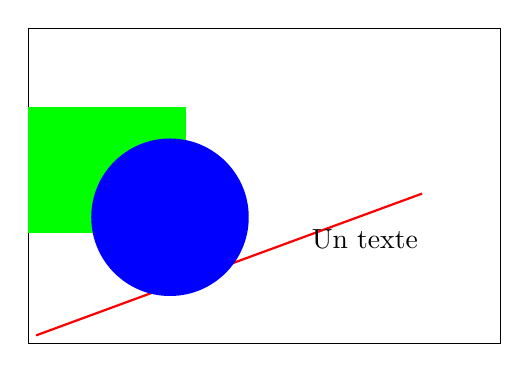
\begin{tikzpicture}[scale=.02]
\draw[thin] (0,0) rectangle (300,200);
\fill[green] (0,70) rectangle ++(100,80);
\draw[red,thick] (5,5)--(250,95);
\fill[blue] (90,80) circle (50);
\node [inner sep=0pt,outer sep=0pt,anchor=south west] at (180,60) {Un texte};
\end{tikzpicture}
    \end{column}
  \end{columns}
  \lstinputlisting[language=XML]{img/06/test.svg}
\end{frame}
\begin{exercice}
  \begin{exercicelet}{Choix de format d'image}
    \begin{questions}
    \item Voici quatre images. Imaginez le format le plus adapté à chacune
      d'entre elles. Expliquez votre choix.\\
      
\includegraphics[width=.2\linewidth]{img/06/tortue.jpg} \hfill
      
\includegraphics[width=.2\linewidth]{img/common/dialog-system.png}
      \hfill
      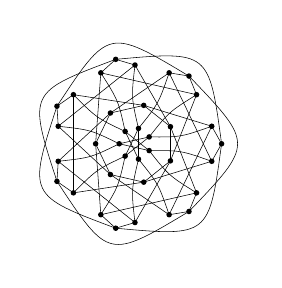
\begin{tikzpicture}[scale=.2,outer sep=0pt, edges/.style={very thin},%
        ]
        \def\vertex#1#2#3{\coordinate #2 at #3;\fill #2 circle (5pt)}%
        \vertex{125}{(noeud1100100)}{(25.63377pt,12.3443pt)};
        \vertex{145}{(noeud1001100)}{(6.33083pt,27.73811pt)};
        \vertex{147}{(noeud1001001)}{(-17.7391pt,22.2439pt)};
        \vertex{347}{(noeud0011001)}{(-28.4523pt,0.0pt)};
        \vertex{367}{(noeud0010011)}{(-17.73868pt,-22.2439pt)};
        \vertex{236}{(noeud0110010)}{(6.3304pt,-27.73856pt)};
        \vertex{256}{(noeud0100110)}{(25.63377pt,-12.34474pt)};
        \vertex{267}{(noeud0100011)}{(61.7215pt,128.16666pt)};
        \vertex{235}{(noeud0110100)}{(-61.7215pt,128.16887pt)};
        \vertex{156}{(noeud1000110)}{(-138.69057pt,31.652pt)};
        \vertex{124}{(noeud1101000)}{(-111.21948pt,-88.69339pt)};
        \vertex{457}{(noeud0001101)}{(0.0pt,-142.2615pt)};
        \vertex{137}{(noeud1010001)}{(111.21948pt,-88.69553pt)};
        \vertex{346}{(noeud0011010)}{(138.69278pt,31.652pt)};
        \vertex{127}{(noeud1100001)}{(15.82706pt,69.34528pt)};
        \vertex{345}{(noeud0011100)}{(-44.34776pt,55.60974pt)};
        \vertex{167}{(noeud1000011)}{(-71.13075pt,0.0pt)};
        \vertex{234}{(noeud0111000)}{(-44.3467pt,-55.60974pt)};
        \vertex{567}{(noeud0000111)}{(15.82599pt,-69.34639pt)};
        \vertex{123}{(noeud1110000)}{(64.08443pt,-30.86185pt)};
        \vertex{456}{(noeud0001110)}{(64.08443pt,30.86075pt)};
        \vertex{467}{(noeud0001011)}{(111.21948pt,88.69339pt)};
        \vertex{237}{(noeud0110001)}{(0.0pt,142.2615pt)};
        \vertex{356}{(noeud0010110)}{(-111.21948pt,88.69553pt)};
        \vertex{126}{(noeud1100010)}{(-138.69278pt,-31.65413pt)};
        \vertex{245}{(noeud0101100)}{(-61.7215pt,-128.16887pt)};
        \vertex{157}{(noeud1000101)}{(61.7215pt,-128.16887pt)};
        \vertex{134}{(noeud1011000)}{(138.69057pt,-31.65413pt)};
        \vertex{135}{(noeud1010100)}{(97.56273pt,122.34378pt)};
        \vertex{146}{(noeud1001010)}{(-34.81718pt,152.56206pt)};
        \vertex{247}{(noeud0101001)}{(-140.98332pt,67.89365pt)};
        \vertex{357}{(noeud0010101)}{(-140.98575pt,-67.89365pt)};
        \vertex{136}{(noeud1010010)}{(-34.81718pt,-152.55962pt)};
        \vertex{246}{(noeud0101010)}{(97.56508pt,-122.34143pt)};
        \vertex{257}{(noeud0100101)}{(156.48766pt,0.0pt)};
        \draw[edges](noeud1100100)--(noeud0011001);
        \draw[edges](noeud1100100)--(noeud0010011); \draw[edges]
        (noeud1100100)..controls (82.98134pt,12.0355pt)..(noeud0011010);
        \draw[edges] (noeud1100100)..controls
        (61.1481pt,57.37003pt)..(noeud0001011);
        \draw[edges](noeud1001100)--(noeud0010011);
        \draw[edges](noeud1001100)--(noeud0110010); \draw[edges]
        (noeud1001100)..controls (42.32513pt,72.38084pt)..(noeud0100011);
        \draw[edges] (noeud1001100)..controls
        (-6.72974pt,83.58076pt)..(noeud0110001);
        \draw[edges](noeud1001001)--(noeud0110010);
        \draw[edges](noeud1001001)--(noeud0100110); \draw[edges]
        (noeud1001001)..controls (-30.19975pt,78.22093pt)..(noeud0110100);
        \draw[edges] (noeud1001001)..controls
        (-69.53915pt,46.84906pt)..(noeud0010110);
        \draw[edges](noeud0011001)--(noeud0100110); \draw[edges]
        (noeud0011001)..controls (-79.98648pt,25.15688pt)..(noeud1000110);
        \draw[edges] (noeud0011001)..controls
        (-79.9874pt,-25.15811pt)..(noeud1100010); \draw[edges]
        (noeud0010011)..controls (-69.53874pt,-46.84798pt)..(noeud1101000);
        \draw[edges] (noeud0010011)..controls
        (-30.19952pt,-78.22096pt)..(noeud0101100); \draw[edges]
        (noeud0110010)..controls (-6.72992pt,-83.58104pt)..(noeud0001101);
        \draw[edges] (noeud0110010)..controls
        (42.32506pt,-72.38211pt)..(noeud1000101); \draw[edges]
        (noeud0100110)..controls (61.14795pt,-57.37129pt)..(noeud1010001);
        \draw[edges] (noeud0100110)..controls
        (82.9804pt,-12.03697pt)..(noeud1011000);
        \draw[edges](noeud0100011)--(noeud0011100);
        \draw[edges](noeud0100011)--(noeud1011000);
        \draw[edges](noeud0100011)--(noeud1010100);
        \draw[edges](noeud0110100)--(noeud1000011);
        \draw[edges](noeud0110100)--(noeud0001011);
        \draw[edges](noeud0110100)--(noeud1001010);
        \draw[edges](noeud1000110)--(noeud0111000);
        \draw[edges](noeud1000110)--(noeud0110001);
        \draw[edges](noeud1000110)--(noeud0101001);
        \draw[edges](noeud1101000)--(noeud0000111);
        \draw[edges](noeud1101000)--(noeud0010110);
        \draw[edges](noeud1101000)--(noeud0010101);
        \draw[edges](noeud0001101)--(noeud1110000);
        \draw[edges](noeud0001101)--(noeud1100010);
        \draw[edges](noeud0001101)--(noeud1010010);
        \draw[edges](noeud1010001)--(noeud0001110);
        \draw[edges](noeud1010001)--(noeud0101100);
        \draw[edges](noeud1010001)--(noeud0101010);
        \draw[edges](noeud0011010)--(noeud1100001);
        \draw[edges](noeud0011010)--(noeud1000101);
        \draw[edges](noeud0011010)--(noeud0100101);
        \draw[edges](noeud1100001)--(noeud0011100);
        \draw[edges](noeud1100001)--(noeud0001110);
        \draw[edges](noeud1100001)--(noeud0010110);
        \draw[edges](noeud0011100)--(noeud1000011);
        \draw[edges](noeud0011100)--(noeud1100010);
        \draw[edges](noeud1000011)--(noeud0111000);
        \draw[edges](noeud1000011)--(noeud0101100);
        \draw[edges](noeud0111000)--(noeud0000111);
        \draw[edges](noeud0111000)--(noeud1000101);
        \draw[edges](noeud0000111)--(noeud1110000);
        \draw[edges](noeud0000111)--(noeud1011000);
        \draw[edges](noeud1110000)--(noeud0001110);
        \draw[edges](noeud1110000)--(noeud0001011);
        \draw[edges](noeud0001110)--(noeud0110001);
        \draw[edges](noeud0001011)--(noeud1010100);
        \draw[edges](noeud0110001)--(noeud1001010);
        \draw[edges](noeud0010110)--(noeud0101001);
        \draw[edges](noeud1100010)--(noeud0010101);
        \draw[edges](noeud0101100)--(noeud1010010);
        \draw[edges](noeud1000101)--(noeud0101010);
        \draw[edges](noeud1011000)--(noeud0100101); \draw[edges]
        (noeud1010100)..controls (-47.76291pt,209.26231pt)..(noeud0101001);
        \draw[edges] (noeud1010100)..controls
        (214.64177pt,0.0026pt)..(noeud0101010); \draw[edges]
        (noeud1001010)..controls (-193.38428pt,93.13577pt)..(noeud0010101);
        \draw[edges] (noeud1001010)..controls
        (133.83827pt,167.81918pt)..(noeud0100101); \draw[edges]
        (noeud0101001)..controls (-193.3816pt,-93.13309pt)..(noeud1010010);
        \draw[edges] (noeud0010101)..controls
        (-47.763pt,-209.25972pt)..(noeud0101010); \draw[edges]
        (noeud1010010)..controls (133.83827pt,-167.8165pt)..(noeud0100101);
      \end{tikzpicture}\hfill
      
\includegraphics[width=.2\linewidth]{img/06/home_organization}

      \begin{xcorrection}
        JPEG (photo), PNG (mais pixelisé) ou vectoriel pour un icone,
        Vectoriel, PNG (peu de couleurs: palette petite, compression idéale,
        dessin au trait pas idéal en JPG).
      \end{xcorrection}
    \end{questions}
  \end{exercicelet}
  \begin{exercicelet}{Palette}
    \begin{questions}
    \item Une image 1000×1000 utilise 3 octets pour décrire la couleur de
      chaque pixel. Calculez la taille occupée par les données de cette image
      en PNG.
      \begin{xcorrection}
        3 Mo
      \end{xcorrection}
    \item Cette image n'a que 256 couleurs au total. On peut utiliser une
      palette de couleurs. Calculez la taille de la palette et la taille des
      données de l'image utilisant la palette.
      \begin{xcorrection}
        1 Mo+768 o pour la palette
      \end{xcorrection}
    \end{questions}
  \end{exercicelet}
\end{exercice}
\subsection{Les couleurs}
\begin{frame}{Qu'est-ce qu'une couleur?}
  \begin{itemize}
  \item Réaction du cerveau à l'intensité des longueurs d'ondes de la lumière
  \item Certaines longueurs d'onde ne sont pas visibles
  \item Le mélange de longueurs d'onde est vu comme une autre couleur.
  \item On n'obtient certaines couleurs que par mélange (rose, marron)
  \item On distingue la couleur d'une source lumineuse, et la couleur d'un
    objet éclairé.
    \begin{itemize}
    \item[\ddialogwarning] Un objet absorbe une partie de la lumière et
      recrache le reste. Par exemple, la chlorophylle absorbe essentiellement
      tout sauf le vert.
    \item Les couleurs d'une source s'additionnent: synthèse additive
    \item Les couleurs de pigments se masquent mutuellement: synthèse
      soustractive
    \end{itemize}
  \end{itemize}
  \begin{center}
    
\includegraphics[width=.8\linewidth]{img/06/Spectrum_roygbiv.jpg}
  \end{center}
\end{frame}
\begin{frame}{Le gamut: teinte et saturation}
  \begin{columns}
    \begin{column}{.5\linewidth}
      \begin{itemize}
      \item Une couleur peut être définie par sa teinte (ou ton), sa
        saturation (intensité de la teinte) et sa luminosité.
      \item Le gamut représente l'étendue des couleurs qui peuvent être
        reproduites par un moniteur ou une imprimante à luminosité fixée
      \item Le polygone représente les couleurs que l'on peut reproduire ; les
        extrémités sont les tons des couleurs de base que l'on mélange.
      \item[\ddialogerror] Certaines couleurs ne peuvent pas être obtenues. On
        perd de l'information lorsqu'on passe d'un système à un autre.
      \item[\ddialoginformation] On utilise des profils couleurs ICC pour
        représenter le gamut et assurer les meilleures conversions possibles.
      \end{itemize}
    \end{column}%
    \begin{column}{.5\linewidth}
      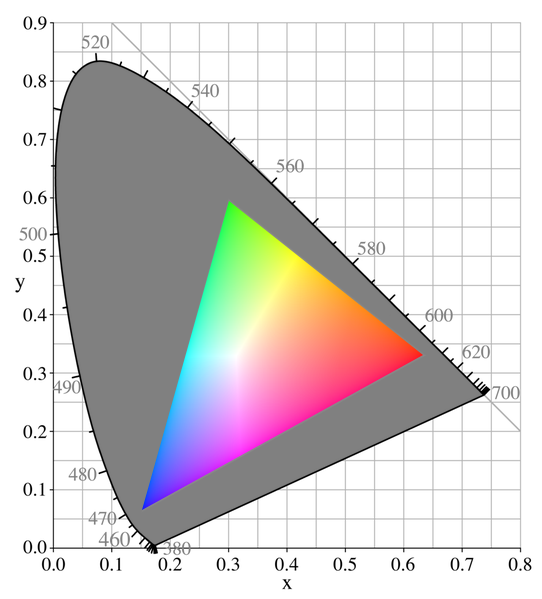
\includegraphics[width=\linewidth]{img/06/CIExy1931_srgb_gamut}
    \end{column}
  \end{columns}
\end{frame}
\begin{frame}{Le gamma: luminance}
  \begin{itemize}
  \item La luminance est l'intensité de la couleur produite
  \item Le facteur $\gamma$ caractérise la réponse lumineuse au stimulus
    électrique: $I=kV^\gamma$.
  \item[\dialogwarning] C'est donc un coefficient d'une réponse exponentielle.
  \end{itemize}
  \begin{center}\renewcommand{\tabcolsep}{1mm}\color{red}
    \begin{tabular}{cccccccccccc}
      Intensité &
      \cellcolor[gray]{.0} 0\%&
      \cellcolor[gray]{.39} 39\%&
      \cellcolor[gray]{.52} 52\%&
      \cellcolor[gray]{.61} 61\%&
      \cellcolor[gray]{.69} 69\%&
      \cellcolor[gray]{.75} 75\%&
      \cellcolor[gray]{.81} 81\%&
      \cellcolor[gray]{.86} 86\%&
      \cellcolor[gray]{.91} 91\%&
      \cellcolor[gray]{.95} 95\%&
      \cellcolor[gray]{1} 100\%\\
      Codage &
      \cellcolor[gray]{.0} 0\% &
      \cellcolor[gray]{.1} 10\% &
      \cellcolor[gray]{.2} 20\% &
      \cellcolor[gray]{.3} 30\% &
      \cellcolor[gray]{.4} 40\% &
      \cellcolor[gray]{.5} 50\% &
      \cellcolor[gray]{.6} 60\% &
      \cellcolor[gray]{.7} 70\% &
      \cellcolor[gray]{.8} 80\% &
      \cellcolor[gray]{.9} 90\% &
      \cellcolor[gray]{1} 100\%\\
    \end{tabular}\\
    \color{solarizedRebase3}\small\itshape
    Signification: lorsque le signal d'entrée est de 10\% de la puissance
    maximale, la perception du gris est de 39\% environ. On compense donc le
    signal entré par le $\gamma$ inverse pour donner l'impression d'une
    progression linéaire.
  \end{center}
  \begin{itemize}
  \item Gamma normalisé des moniteurs: 2,5
  \item[\dialogerror] Mais... tous les moniteurs n'ont pas le même $\gamma$.
  \item Nécessité de corriger la correction (on fait le produit des $\gamma$).
  \end{itemize}
\end{frame}
\begin{frame}[fragile]{Images RVB (RGB en anglais)}
  \begin{columns}
    \begin{column}{.6\linewidth}
      \begin{itemize}
      \item Le standard est de recomposer la couleur par synthèse additive de
        3 couleurs.
      \item On mesure les couleurs par l'intensité de chacune des couleurs
        primaires: rouge, vert et bleu
      \item On obtient des couleurs par mélange de différentes intensités de
        RVB
      \item Un système équivalent permet de désigner les couleurs par teinte,
        saturation et luminance relative (valeur): TSV (en anglais HSB,
        Hue/Saturation/Brightness).
      \item On utilise très souvent un octet d'information pour chaque
        composante.
      \item Notation usuelle: \#RRVVBB (avec chaque paire de lettre qui est un
        octet noté en hexadécimal).
      \end{itemize}
    \end{column}%
    \begin{column}{.4\linewidth}\centering
      \begin{tikzpicture}[scale=.5]
        \foreach \x in {0,0.0111,...,1} { \definecolor{currentcolor}{hsb}{\x,
            1, 1} \draw[draw=none, fill=currentcolor] (-360*\x+88:2) --
          (-360*\x+88:3.8) -- (-360*\x+92:3.8) -- (-360*\x+92:2) -- cycle; }
        \foreach \x/\y in
        {0/rouge,60/jaune,120/vert,180/cyan,240/bleu,300/magenta} { \draw
          [black] (90-\x:3.8)--(90-\x:5); \draw [decorate,decoration={text
            along path, text=\x{°}/\y}] (88-\x:4) arc (88-\x:28-\x:4); }
      \end{tikzpicture}
      \\
      La roue des couleurs permet d'identifier la teinte à saturation
      maximale.
    \end{column}
  \end{columns}
\end{frame}
\begin{exercice}
  \begin{exercicelet}{Décomposition de couleurs}
    Donnez des composantes couleur plausibles RGB des couleurs
    suivantes. Utilisez la notation HTML.
    \begin{itemize}
    \item Rouge, vert, bleu
    \item Cyan, magenta, jaune
    \item Blanc, noir
    \item Gris 50\%
    \item Marron foncé, rose pâle, orange vif
    \end{itemize}
    \begin{xcorrection}
      FF0000, 00FF00, 0000FF\\
      00FFFF, FF00FF, FFFF00\\
      FFFFFF, 000000\\
      808080\\
      200000 (ou autre faible quantité de rouge), FFE0E0 (rouge un peu plus
      que les autres, mais très blanc), FF7F00 (ou autre chose équivalente:
      mélange jaune+rouge)
    \end{xcorrection}
  \end{exercicelet}
  \begin{exercicelet}{Scanner}
    Un scanner scanne en RGB à une résolution de 1200 points par pouce (dans
    les deux directions). Pour simplifier, on considérera qu'il y a une
    surface de 10 pouces × 6 pouces scannable. Chaque couleur est scannée en
    12 bits. Quelle est la quantité d'information résultant de chaque scan ?
    \begin{xcorrection}
      1200×1200×60×12×3=3 110 400 000 soit environ 389 Mo.
    \end{xcorrection}
  \end{exercicelet}
\end{exercice}
\begin{frame}{Images CMJN et polychromes}
  \begin{columns}
    \begin{column}{.8\linewidth}
      \begin{itemize}
      \item L'impression utilise un standard de synthèse soustractive
      \item Deux pigments ensemble absorbent tous les deux la lumière et dans
        l'absolu le mélange complet fait du noir.
      \item[\dialogerror] Le noir par addition n'est pas assez noir, on
        utilise donc une encre noire pure.
      \item Utilisation des couleurs complémentaires cyan, magenta et jaune
      \item Standard de l'impression: la \emph{quadrichromie} CMJN (CMYK en
        anglais).
      \item[\dialogerror] Certaines teintes ne sont pas possibles: rose vif,
        oranges vifs.
      \item Possibilité d'impression pentachrome ou hexachrome
      \item[\ddialogwarning] possibilité de faire des couleurs garanties avec
        une encre par couleur sans mélanges: gamme Pantone® ou Focoltone®.
      \end{itemize}
    \end{column}%
    \begin{column}{.15\linewidth}\centering
      
\includegraphics[width=\linewidth]{img/06/lena-CMJN-cyan}\\
      
\includegraphics[width=\linewidth]{img/06/lena-CMJN-magenta}\\
      
\includegraphics[width=\linewidth]{img/06/lena-CMJN-jaune}\\
      
\includegraphics[width=\linewidth]{img/06/lena-CMJN-noir}\\
    \end{column}
  \end{columns}
\end{frame}
\begin{exercice}
  \begin{exercicelet}{Conversion HTML-CMJ}
    La trichromie consiste à n'utiliser que trois couleurs et faire le noire
    par mélange des autres couleurs. Dans ce cas, la formule est simple: la
    proportion d'une encre est 100\% - la proportion de la couleur
    complémentaire.

    Convertissez la couleur suivante en CM: \#FA0140. Quel genre de teinte
    est-ce ?  Est-elle très saturée ?
    \begin{xcorrection}
      FFFFFF-FA0140=05FEBF en CMJ. Elle est assez saturée (beaucoup d'encre
      magenta et pas mal de jaune). C'est quelque chose assez rouge (un peu
      violacé).
    \end{xcorrection}
  \end{exercicelet}
  \begin{exercicelet}{Vitesse d'impression}
    Une imprimante en quadrichromie est capable d'imprimer 6 pages par
    minutes, en 1200 points par pouce en mode RVB 8 bits par composante. Pour
    simplifier, on considérera qu'il y a une surface de 10 pouces × 6 pouces
    imprimable. Quelle est la quantité d'information qu'on doit fournir à
    l'imprimante pour une page ? Pour une minute d'impression ?
    \begin{xcorrection}
      Même chose que précédemment, mais seulement 8 bits, donc chaque page
      représente : 259 200 000 octets, soit environ 1,5 Go par minute.
    \end{xcorrection}
  \end{exercicelet}
\end{exercice}
\subsection{Les sons}
\begin{frame}{Qu'est-ce qu'un son?}
  Un son est une vibration de l'air transportant un signal. C'est aussi le
  signal véhiculé par vibration.

  Le son est donc numérisé comme vu au chapitre 1. Il est caractérisé par son
  spectre de fréquence instantané (les sons purs et périodiques qui le
  constituent à un moment donné). Un son est venu, à un instant donné, comme
  la somme de plusieurs sons «~purs~».
  
  La reproduction du son se fait en reproduisant une vibration qui a les mêmes
  caractéristiques fréquentielles. Les données audio sont donc des variations
  de pression (ou plutôt d'intensité électrique dans les capteurs et
  émetteurs).
\end{frame}
\begin{frame}{Les formats}
  \begin{itemize}
  \item Il faut distinguer les formats de fichiers des codecs (méthode de
    compression et filtrage des données).
  \item On distingue trois types de formats:
    \begin{enumerate}
    \item Des formats non compressés qui rajoutent quelques méta-données (ou
      pas) à des données brutes (WAV, PCM, AIFF)
    \item Des formats compressés qui utilisent un algorithme (le \emph{codec})
      pour compresser et éventuellement réduire la quantité d'information avec
      une perte acceptable de qualité (FLAC, MP3, AAC, OGG)
    \item Des formats synthétiques qui contiennent des données d'instruments
      pour reproduire de la musique à base d'une partition (MIDI, SID)
    \end{enumerate}
  \item[\ddialogwarning] Dans le domaine de la musique, le codec sert rarement
    à plusieurs formats (aucun obstacle théorique) à part PCM (pas de
    compression)
  \end{itemize}
  \begin{block}{Caractéristiques}
    Le débit d'information va dépendre:
    \begin{itemize}
    \item Du nombre de voies (émetteurs indépendants pour reconstituer
      l'aspect spatial)
    \item Des fréquences reproduites (théorème d'échantillonage)
    \item De la quantification désirée (en nombre de bits)
    \end{itemize}
  \end{block}
\end{frame}
\begin{exercice}
  \begin{exercicelet}{Compression audio MP3}
    Le codec MP3 permet de compresser le signal sonore dans une grande variété
    de débits finaux (après compression), le plus commun étant 128 kb/s. La
    fréquence d'échantillonage est quasi-toujours 44,1
    kHz. \textbf{Calculatrice autorisée}.
    \begin{questions}
    \item Quel est le débit non compressé pour de l'audio stéréo 16 bits ?
      \begin{correction}
        16 bit/sample × 44100 samples/second × 2 channels / 1000
        bits/kilobit=1411,2 kb/s.
      \end{correction}
    \item Quel est le taux de compression du format MP3 le plus classique
      (débit final 128 kb/s) ?
      \begin{correction}
        1411,2/128=11,02 (et des poussières)
      \end{correction}
    \item Et avec le format plus généreux à 320 kb/s au final?
      \begin{correction}
        1411,2/320=4,41
      \end{correction}
    \end{questions}
  \end{exercicelet}
\end{exercice}
\subsection{Les films}
\begin{frame}{Qu'est-ce qu'un film?}
  \begin{itemize}
  \item Un film est toute sorte d'image animée synchronisée ou non avec du son
    ou du texte.
  \item[\dialogwarning] Ils représentent plus de la moitié du trafic
    nord-américain sur internet.
  \item Les images successives s'appellent des trames (anglais \emph{frames}).
  \item La synchronisation avec le son doit être précise et résistante aux
    erreurs.
  \end{itemize}
\end{frame}
\begin{frame}{Les containers et les codecs}
  \begin{itemize}
  \item Comme pour l'audio, on distingue les formats (AVI, MP4, MPEG, MOV,
    MKS) des codecs (DIVX, x264, Theora, FFMPEG, Sorenson)
  \item Un certain nombre de formats n'acceptent qu'un nombre restreint de
    codecs vidéos ou audios (MP4 par exemple).
  \item Le processus administratif de normalisation pèse très lourd, car les
    fabriquants doivent faire du matériel conforme
  \item Les DRM sont des protections rajoutées qui empêchent dans certaines
    (nombreuses) circonstances d'accéder aux données. Elles sont dépendantes
    d'une inviolabilité du matériel et du logiciel.
  \item Citons aussi les GIF animés (et APNG) qui sont des formats d'images
    permettant une animation simple
  \item Ces formats peuvent contenir des méta-données plus ou moins riches
    (titre, auteurs, DRM,\dots).
  \end{itemize}
\end{frame}
\begin{frame}{L'encodage}
  \begin{itemize}
  \item La phase d'encodage d'une vidéo ou d'un fichier audio consiste à
    repérer les similarités entre plusieurs trames successives.
  \item On peut par exemple décider s'il vaut mieux décrire les différences ou
    envoyer une nouvelle image.
  \item Deux images très similaires peuvent être compressées par exemple en
    faisant un XOR binaire entre les deux et en compression RLE après.
  \item Les codecs font aussi du filtrage perceptuel pour réduire la quantité
    de données. La compression peut-être plus agressive lorsque l'autre
    méthode donne de mauvais résultats.
  \item Il est important de garder des trames complètes périodiquement pour
    gérer les erreurs.
  \item Encodage souvent en deux passes (estimation des débits binaires
    voulus, puis calcul définitif)
  \item Actuellement, l'une des opérations les plus coûteuses en temps de
    calcul.
  \item Certains formats spéciaux multi-débits permettent de s'adapter à la
    vitesse de communication de deux ordinateurs pour proposer la meilleure
    qualité \emph{(streaming)}.
  \end{itemize}
\end{frame}

% Local Variables:
% TeX-master: "archi06"
% TeX-PDF-mode: t
% fill-column: 78
% coding: utf-8-unix
% mode-require-final-newline: t
% mode: latex
% mode: flyspell
% ispell-local-dictionary: "francais"
% End:

\appendix
  \subsection{Le jeu du fakir}
  \begin{frame}[label=fakira]
    \frametitle{Le jeu du fakir (1)}
    Est-ce que le nombre choisi est impair ?
  \end{frame}
  \begin{frame}[label=fakirb]
    \frametitle{Le jeu du fakir (2)}
    Est-ce que le nombre choisi fait partie de ceux-ci:
    \begin{tabular}{|c|c|c|c|c|c|c|c|c|c|}\hline
      2&3&6&7&10&11&14&15\\\hline
      18&19&22&23&26&27&30&31\\\hline
      34&35&38&39&42&43&46&47\\\hline
      50&51&54&55&58&59&62&63\\\hline
      66&67&70&71&74&75&78&79\\\hline
      82&83&86&87&90&91&94&95\\\hline
      98&99&&&&&&\\\hline
    \end{tabular}
  \end{frame}
  \begin{frame}[label=fakirc]
    \frametitle{Le jeu du fakir (3)}
    Est-ce que le nombre choisi fait partie de ceux-ci:
    \begin{tabular}{|c|c|c|c|c|c|c|c|c|c|}\hline
      4&5&6&7&12&13&14&15\\\hline
      20&21&22&23&28&29&30&31\\\hline
      36&37&38&39&44&45&46&47\\\hline
      52&53&54&55&60&61&62&63\\\hline
      68&69&70&71&76&77&78&79\\\hline
      84&85&86&87&92&93&94&95\\\hline
      100&&&&&&&\\\hline
    \end{tabular}
  \end{frame}
  \begin{frame}[label=fakird]
    \frametitle{Le jeu du fakir (4)}
    Est-ce que le nombre choisi fait partie de ceux-ci:
    \begin{tabular}{|c|c|c|c|c|c|c|c|c|c|}\hline
      8&9&10&11&12&13&14&15\\\hline
      24&25&26&27&28&29&30&31\\\hline
      40&41&42&43&44&45&46&47\\\hline
      56&57&58&59&60&61&62&63\\\hline
      72&73&74&75&76&77&78&79\\\hline
      88&89&90&91&92&93&94&95\\\hline
    \end{tabular}
  \end{frame}
  \begin{frame}[label=fakire]
    \frametitle{Le jeu du fakir (5)}
    Est-ce que le nombre choisi fait partie de ceux-ci:
    \begin{tabular}{|c|c|c|c|c|c|c|c|c|c|}\hline
      16&17&18&19&20&21&22&23\\\hline
      24&25&26&27&28&29&30&31\\\hline
      48&49&50&51&52&53&54&55\\\hline
      56&57&58&59&60&61&62&63\\\hline
      80&81&82&83&84&85&86&87\\\hline
      88&89&90&91&92&93&94&95\\\hline
    \end{tabular}
  \end{frame}
  \begin{frame}[label=fakirf]
    \frametitle{Le jeu du fakir (6)}
    Est-ce que le nombre choisi fait partie de ceux-ci:
    \begin{tabular}{|c|c|c|c|c|c|c|c|c|c|}\hline
      32&33&34&35&36&37&38&39\\\hline
      40&41&42&43&44&45&46&47\\\hline
      48&49&50&51&52&53&54&55\\\hline
      56&57&58&59&60&61&62&63\\\hline
      96&97&98&99&100&&&\\\hline
    \end{tabular}
  \end{frame}
  \begin{frame}[label=fakirg]
    \frametitle{Le jeu du fakir (7)}
    Est-ce que le nombre choisi est strictement plus grand que 63 ?\pause

    {\large Le nombre est...}
    \hyperlink{mesure}{\beamergotobutton{Retour}}
  \end{frame}

% Local Variables:
% TeX-master: "archi01"
% TeX-PDF-mode: t
% fill-column: 78
% coding: utf-8-unix
% mode-require-final-newline: t
% mode: latex
% mode: flyspell
% ispell-local-dictionary: "francais"
% End:

\subsection{La table ASCII}
\begin{frame}[label=ascii]{La table ASCII}
  \begin{itemize}
  \item 32 caractères de «~contrôle~», 96 «~affichables~»;
  \item Unicode, ISO-8859 compatibles avec ASCII.
  \end{itemize}
  \textcolor{solarizedRebase3}{\fontsize{8}{8}\ttfamily\selectfont
    \rowcolors{1}{solarizedRebase02}{solarizedRebase03}%
    \begin{tabular}{|l|l|l|l|l|l|l|l|}\hline
      00~NUL&01~SOH&02~STX&03~ETX&04~EOT&05~ENQ&06~ACK&07~BEL\\
      08~BS~&09~HT~&0A~NL~&0B~VT~&0C~NP~&0D~CR~&0E~SO~&0F~SI~\\
      10~DLE&11~DC1&12~DC2&13~DC3&14~DC4&15~NAK&16~SYN&17~ETB\\
      18~CAN&19~EM~&1A~SUB&1B~ESC&1C~FS~&1D~GS~&1E~RS~&1F~US~\\\hline
      20~SP~&21~~\string!~&22~~"~&23~~\#~&24~~\$~&25~~\%~&26~~\&~&27~~'~\\
      28~~(~&29~~)~&2A~~*~&2B~~+~&2C~~,~&2D~~-~&2E~~.~&2F~~/~\\
      30~~0~&31~~1~&32~~2~&33~~3~&34~~4~&35~~5~&36~~6~&37~~7~\\
      38~~8~&39~~9~&3A~~\string:~&3B~~\string;~&3C~~<~&3D~~=~&3E~~>~&3F~~\string?~\\
      40~~@~&41~~A~&42~~B~&43~~C~&44~~D~&45~~E~&46~~F~&47~~G~\\
      48~~H~&49~~I~&4A~~J~&4B~~K~&4C~~L~&4D~~M~&4E~~N~&4F~~O~\\
      50~~P~&51~~Q~&52~~R~&53~~S~&54~~T~&55~~U~&56~~V~&57~~W~\\
      58~~X~&59~~Y~&5A~~Z~&5B~~[~&5C~~\textbackslash~&5D~~]~&5E~~\string^~&5F~~\_~\\
      60~~`~&61~~a~&62~~b~&63~~c~&64~~d~&65~~e~&66~~f~&67~~g~\\
      68~~h~&69~~i~&6A~~j~&6B~~k~&6C~~l~&6D~~m~&6E~~n~&6F~~o~\\
      70~~p~&71~~q~&72~~r~&73~~s~&74~~t~&75~~u~&76~~v~&77~~w~\\
      78~~x~&79~~y~&7A~~z~&7B~~\{~&7C~~\string|~&7D~~\}~&7E~~\string~~&7F~DEL\\%
      \hline
    \end{tabular}}
  \hyperlink{jeucaractere}{\beamergotobutton{Retour}}
\end{frame}


\end{document}

% Local Variables:
% TeX-master: "archi01"
% TeX-PDF-mode: t
% fill-column: 78
% coding: utf-8-unix
% mode-require-final-newline: t
% mode: latex
% mode: flyspell
% ispell-local-dictionary: "francais"
% End:

\end{document}

% Local Variables:
% TeX-master: "archi"
% TeX-PDF-mode: t
% fill-column: 78
% coding: utf-8-unix
% mode-require-final-newline: t
% mode: latex
% mode: flyspell
% ispell-local-dictionary: "francais"
% End:
